% ****** Start of file apssamp.tex ******
%
%   This file is part of the APS files in the REVTeX 4.2 distribution.
%   Version 4.2a of REVTeX, December 2014
%
%   Copyright (c) 2014 The American Physical Society.
%
%   See the REVTeX 4 README file for restrictions and more information.
%
% TeX'ing this file requires that you have AMS-LaTeX 2.0 installed
% as well as the rest of the prerequisites for REVTeX 4.2
%
% See the REVTeX 4 README file
% It also requires running BibTeX. The commands are as follows:
%
%  1)  latex apssamp.tex
%  2)  bibtex apssamp
%  3)  latex apssamp.tex
%  4)  latex apssamp.tex
%
\documentclass[
reprint,
superscriptaddress,
% groupedaddress,
% unsortedaddress,
% runinaddress,
%frontmatterverbose, 
%preprint,
%preprintnumbers,
nofootinbib,
%nobibnotes,
%bibnotes,
amsmath,amssymb,
aps,
%rmp,
%prstab,
%prstper,
%floatfix,
prd,
]{revtex4-2}

\usepackage{graphicx}% Include figure files
\usepackage{dcolumn}% Align table columns on the decimal point
\usepackage{bm}% bold math
%\usepackage{ctex}
\usepackage{gensymb}
\usepackage{subfigure}
\usepackage{amsmath,siunitx}
\usepackage{hyperref}% add hypertext capabilities
\usepackage{booktabs, multirow}

% \allowdisplaybreaks

%\usepackage{pdfpages}
% \usepackage{cuted}

%\usepackage[mathlines]{lineno}% Enable numbering of text and display math
%\linenumbers\relax % Commence numbering lines

%\usepackage[showframe,%Uncomment any one of the following lines to test 
%%scale=0.7, marginratio={1:1, 2:3}, ignoreall,% default settings
%%text={7in,10in},centering,
%%margin=1.5in,
%%total={6.5in,8.75in}, top=1.2in, left=0.9in, includefoot,
%%height=10in,a5paper,hmargin={3cm,0.8in},
%]{geometry}

\begin{document}

\preprint{APS/123-QED}

\title{The study of non-complete-ring positron emission tomography (PET) detection method}% Force line breaks with \\
%\thanks{A footnote to the article title}%

% \author{Yeqi Fang$^{1}$}
% \email{fangyeqi@stu.scu.edu.cn}
% \author{Wei Hong$^{2}$}
% \email{weihong@mail.bnu.edu.cn}
% \author{Jun Tao$^{1}$}
% \email{taojun@scu.edu.cn, corresponding author}

% \affiliation{$^{1}$Center for Theoretical Physics, College of Physics, Sichuan University, Chengdu, 610065, China}
% \affiliation{$^{2}$Department of Astronomy, Beijing Normal University, Beijing 100875, People's Republic of China}
\author{Yeqi Fang}
\email{fangyeqi@stu.scu.edu.cn}
\affiliation{College of Physics, Sichuan University, Chengdu, 610065, China}

\author{Rong Zhou}
\email{zhourong@scu.edu.cn}
\affiliation{College of Physics, Sichuan University, Chengdu, 610065, China}

%\collaboration{MUSO Collaboration}%\noaffiliation

%\date{\today}% It is always \today, today,
%  but any date may be explicitly specified

\begin{abstract}
	Positron Emission Tomography (PET) is a vital molecular imaging tool widely used in medical diagnosis and treatment evaluation. Traditional PET systems typically rely on complete detector rings to achieve full angular coverage for uniform and statistically robust sampling of coincidence events. However, incomplete-ring PET scanners have emerged in various scenarios due to hardware failures, cost constraints, or specific clinical needs. In such cases, conventional reconstruction algorithms often suffer from performance degradation due to reduced data completeness and geometric inconsistencies. This thesis proposes a coarse-to-fine reconstruction framework for incomplete-ring PET scanners. The framework first employs an Attention U-Net model to recover complete sinograms from incomplete ones, then uses the OSEM algorithm for preliminary reconstruction, and finally applies a two-stage architecture comprising a Coarse Prediction Module (CPM) and an Iterative Refinement Module (IRM) for fine reconstruction. Our approach utilizes neighboring axial slices and spectral transform features as auxiliary guidance at the input level to ensure spatial and frequency domain consistency, and integrates a contrastive diffusion strategy at the output level to improve correspondence between low-quality PET inputs and refined PET outputs. Experimental results on public and in-house brain PET datasets demonstrate that the proposed method significantly outperforms existing approaches in metrics such as PSNR (35.6421 dB) and SSIM (0.9588), successfully preserving key anatomical structures and tracer distribution features, thus providing an effective solution for incomplete-ring PET imaging.
\end{abstract}
% \newpage
% \tableofcontents
%\keywords{Suggested keywords}%Use showkeys class option if keyword
%display desired
\maketitle

%\tableofcontents

%!TEX root = ../Manual.tex
\section{Introduction}
\label{chap:introduction}

\subsection{Background and Motivation}


Positron emission tomography (PET) is a molecular imaging modality that provides quantitative in vivo visualization of metabolic processes  \cite{townsend2004}. In PET, a radiotracer decays by positron emission; each positron annihilates with an electron to produce a pair of $511$keV photons traveling in nearly opposite directions. These annihilation photons are detected in coincidence by a ring of scintillation detectors, with each coincident detection defining a line-of-response (LOR). Conventional PET scanners employ a complete 360$^\circ$ detector ring to maximize sensitivity and ensure uniform angular coverage  \cite{townsend2004}.

However, building full-ring PET scanners may sometimes be impractical. \textbf{Incomplete-ring PET systems} have been developed for various practical reasons: reducing cost and complexity, allowing closer patient access in dedicated breast scanners  \cite{surti2008}, creating "open" configurations for interventions or reducing claustrophobia  \cite{tashima2012, krishnamoorthy2021}, and enabling specialized applications like dual-panel systems for brain imaging  \cite{zhang2020}. While these systems expand PET's utility, the incomplete angular coverage leads to missing projection data and an underdetermined reconstruction problem. Classical tomographic theory dictates that missing angular views introduce artifacts and non-uniform resolution  \cite{kak1988, surti2008}. Even with time-of-flight capabilities that partially compensate for limited view angles  \cite{surti2008, krishnamoorthy2021}, incomplete-ring PET data remain challenging to reconstruct with high fidelity.

Multiple reconstruction approaches have been investigated for incomplete-ring PET. Analytical methods like filtered back-projection assume complete data and produce pronounced streak artifacts with incomplete rings  \cite{kak1988}. Iterative reconstruction algorithms such as maximum-likelihood expectation-maximization (MLEM) better accommodate incomplete data by modeling the acquisition process  \cite{qi2006}, but still suffer from artifacts along missing view directions  \cite{zhang2020}. Penalized likelihood methods incorporating prior constraints can reduce these artifacts, as demonstrated by Zhang \textit{et al.} using a high-quality prior image to improve contrast recovery in a dual-panel head-and-neck PET system  \cite{zhang2020}.

In recent years, deep learning techniques have emerged as powerful tools for PET reconstruction. Regression-based networks have shown effectiveness in tasks such as low-dose PET denoising and partial data reconstruction  \cite{Kandarpa_2021}, learning direct mappings from degraded to high-quality images. Liu \textit{et al.} demonstrated that a U-Net architecture could transform artifact-degraded partial-ring PET images into more complete images  \cite{liu2019}, though CNNs often struggle with global features when facing large-scale angular losses. 
Unsupervised and physics-guided methods like Shan \textit{et al.}'s deep image prior approach can optimize a network to match measured projections without external training pairs  \cite{shan2024}. GAN-based methods generate visually reasonable images by inferring missing structures  \cite{xue2023cg3dsrganclassificationguided3d}, though training instability and quantitative accuracy remain concerns. Likelihood-based generative models like VAEs and normalizing flows operate within a more rigorous theoretical framework but often produce blurry results with high computational complexity. Advanced approaches including model-based deep learning frameworks and generative models have shown promise for enhancing PET reconstructions  \cite{reader2023, vashistha2024}, but must be applied carefully to ensure no clinically important detail is hallucinated or lost.

Despite these advances, significant challenges persist for incomplete-ring PET imaging due to fundamental \textbf{information loss}. Analytical methods cannot adequately handle data deficiency, over-regularized iterative methods might erase subtle features, and deep learning models risk introducing bias. Current approaches either cannot effectively handle large-scale data loss, have excessive computational overhead, or struggle to maintain the detailed features required for clinical diagnosis. In response, this thesis proposes an innovative coarse-to-fine diffusion model framework that is computationally efficient, stable in performance, and optimized specifically for incomplete ring PET scanners, aiming to recover missing angular information and suppress reconstruction artifacts without sacrificing true image detail.



\begin{figure}[htbp]
	\centering
	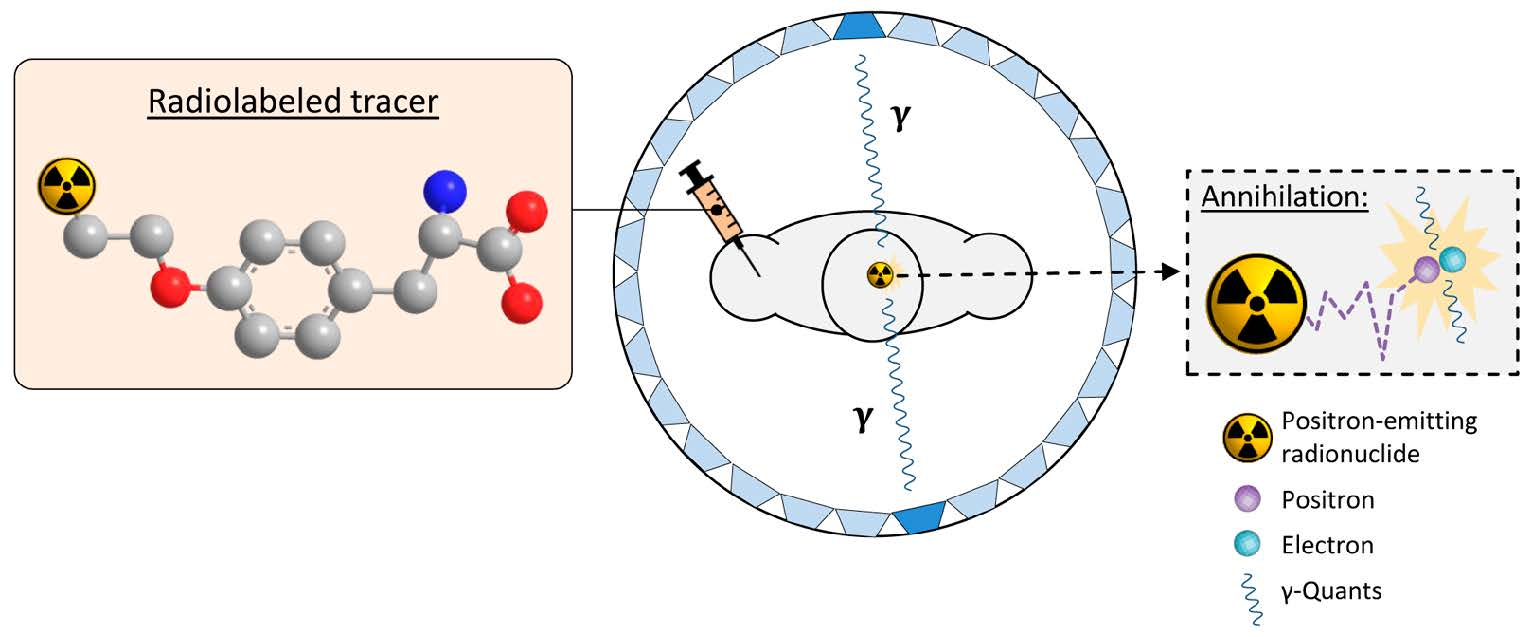
\includegraphics[scale=0.47]{./Images/graph.jpg}
	\caption{Principles of Positron Emission Tomography (PET) imaging.}
	\label{fig:graph}
\end{figure}




% \subsection{Thesis Organization}
The remainder of this thesis is organized as follows:

\textbf{Section \ref{chap:background}} (\emph{Background on PET Imaging and Incomplete Ring Geometry}) provides an overview of PET physics, principles of coincidence detection, and the main challenges introduced by incomplete rings. We also summarize classical and modern reconstruction methods.

\textbf{Section \ref{chap:methods}} (\emph{Fundamentals of Diffusion Probabilistic Models}) details the background of Denoising Diffusion Probabilistic Models (DDPM) and how they apply to various image reconstruction tasks, establishing the theoretical foundation for our proposed method. \emph{Proposed Coarse-to-Fine Reconstruction Framework}) describes the detailed workflow of our method, including complete and incomplete ring geometric modeling, creation of list-mode and sinogram data, the coarse-to-fine design, auxiliary guidance modules, contrastive diffusion learning objectives, and implementation details.

\textbf{Section \ref{chap:results}} (\emph{Experiments and Results}) presents our extensive experimental setups, hyperparameter choices, evaluation metrics, ablation studies, and comparisons with state-of-the-art methods. We also present results of cross-dataset evaluation on in-house datasets.

\textbf{Section \ref{chap:conclusion}} (\emph{Conclusion and Future Work}) summarizes our findings, discusses limitations, and suggests directions for future research, including potential improvements for real-world incomplete ring PET scanners.

\textbf{Appendices} provide additional experiments, extended qualitative results, and tables of hyperparameters used in the thesis.

% \section{APPENDIX}\label{appendix:model}

%!TEX root = ../Manual.tex
\section{Background on PET Imaging and Incomplete Ring Geometry}
\label{chap:background}


This section provides a brief but comprehensive overview of the fundamental aspects of PET imaging, focusing on the detection process, data acquisition methods, and conventional reconstruction algorithms. We then discuss incomplete ring PET scanners in detail, highlighting the geometry of missing detectors, their impact on data quality, and current solutions and unresolved research challenges.

\subsection{Principles of PET Imaging}
In PET imaging, positron-emitting nuclides (typically $^{18}\text{F}$, $^{15}\text{O}$, $^{11}\text{C}$, etc.) are usually combined with biologically relevant tracer compounds. After entering the bloodstream, these nuclides decay, with each emitting a positron. When the positron encounters an electron, an annihilation event occurs, producing two gamma photons, each with an energy of approximately 511 keV, traveling in nearly opposite directions (collinearly).

\begin{figure*}[htbp]
    \centering
    \vspace{-0.2cm}
    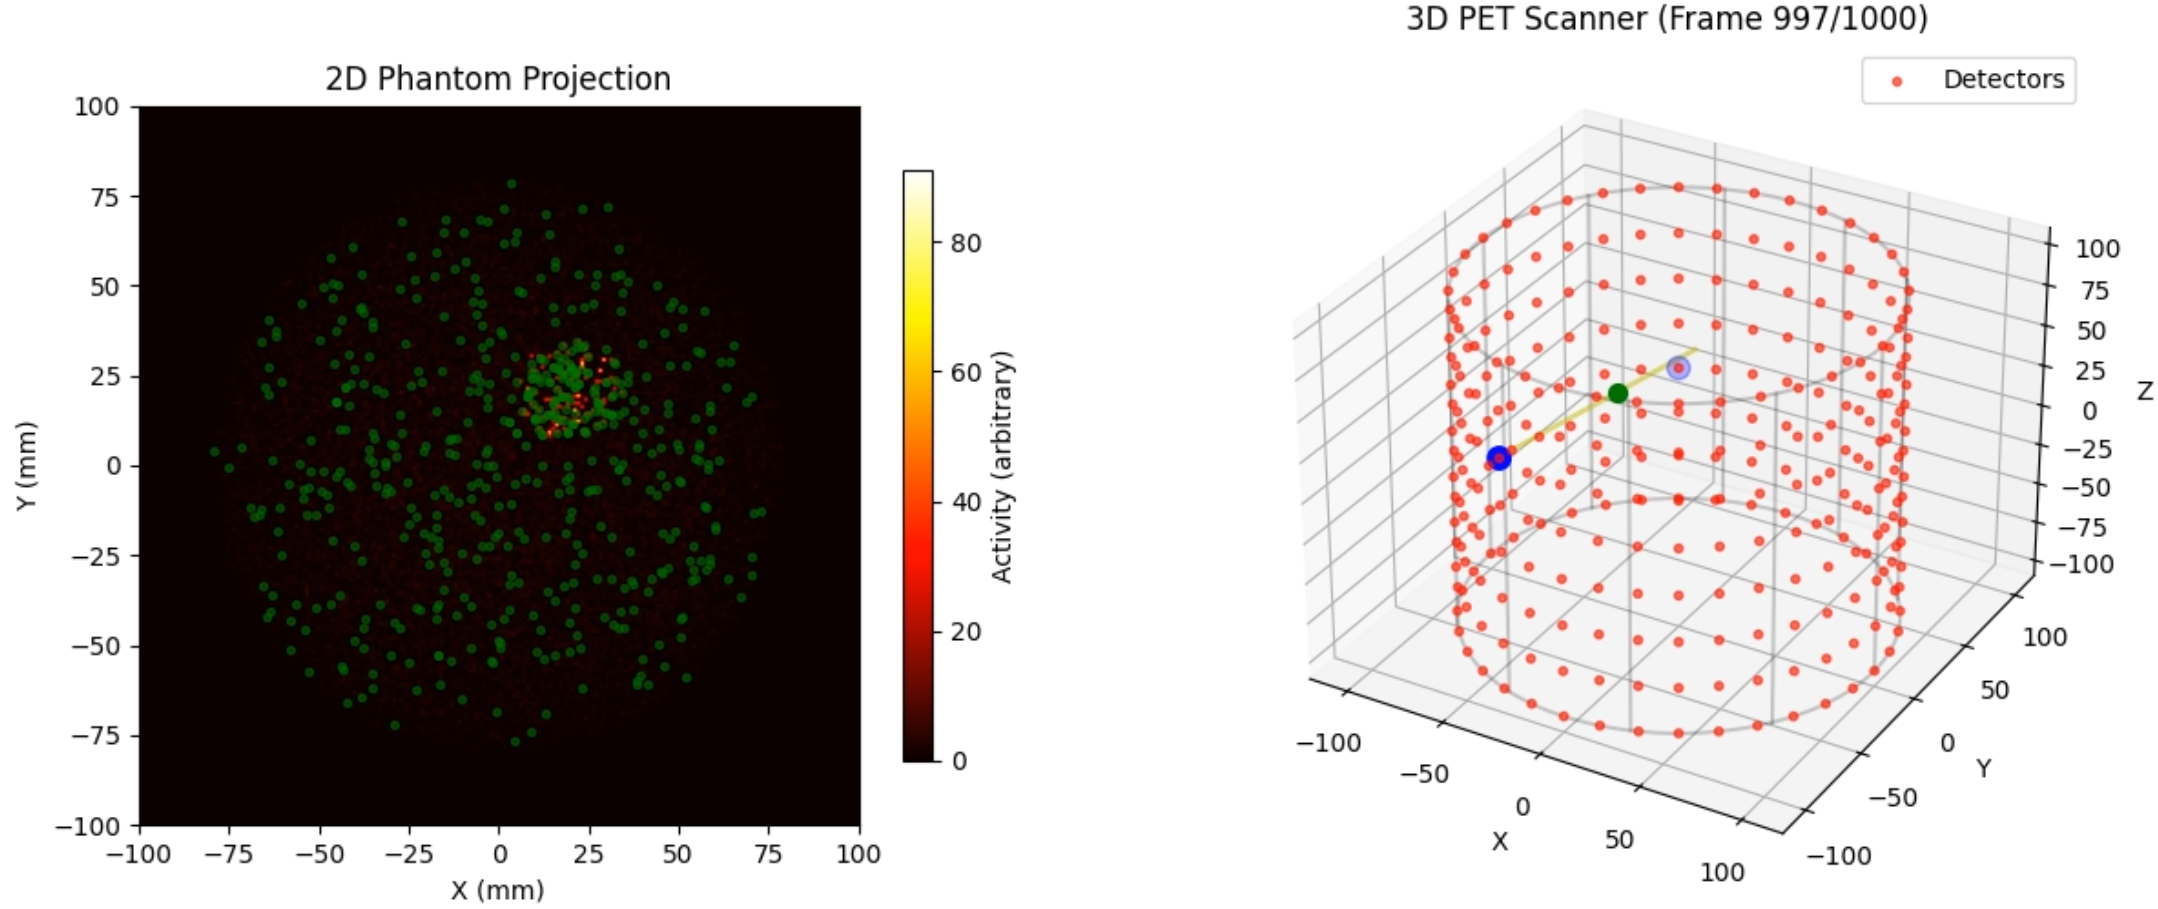
\includegraphics[width=0.98\textwidth]{Images/Screenshot2025-02-07214940}
    \vspace{-0.2cm}
    \caption{Schematic diagram of PET detection, where the red dot represents the detector center, the green dot represents the annihilation event location, and the two blue dots represent the centers of the two detectors that detect the gamma rays. This figure is only illustrative; the detector parameters in the figure do not equal the actual simulation parameters.}
    \vspace{-0.2cm}
    \label{fig:pet_event}
\end{figure*}

PET scanners are designed to detect coincidences of these 511 keV photon pairs. When two detectors at different positions record gamma photons within a short coincidence time window, it is assumed that these photons came from the same annihilation event. This forms a line of response (LOR) between the two detector elements, as shown in Figure~\ref{fig:pet_event}.
PET data can be acquired in multiple formats:
(1) \textbf{List-mode data}: Each coincidence event is recorded individually, providing precise detector pair identification and timestamps.
(2) \textbf{Sinogram data}: By categorizing coincidence counts into projection bins indexed by radial, angular, and axial coordinates (possibly also by axial ring difference), forming a 2D (or 3D) histogram.
In a typical 3D PET system, a scanner with a complete ring covers a 360$^\circ$ view angle around the patient, ensuring uniform sampling of LORs.

\subsection{Incomplete Ring PET Scanners}

In normal PET (Positron Emission Tomography) system design, \emph{incomplete rings} or \emph{partial rings} often arise from various practical considerations and technical constraints. From an economic perspective, reducing the total number of detectors can effectively lower system costs. In certain specialized fields, such as brain imaging or organ-specific examinations, researchers may adopt partially covered designs to accommodate smaller field-of-view requirements. Additionally, with the continuous development of medical technology, innovative designs for hybrid or portable PET are increasingly important; these systems meet the needs of different clinical and research scenarios through lightweight, flexible structures. It is worth noting that technical factors such as detector failures, maintenance, upkeep, calibration, and other issues may also cause certain ring segments to temporarily stop operating, resulting in incomplete detector rings. These variations reflect the complexity and adaptability of PET imaging technology in practical applications.


The main difficulty with incomplete rings is the reduction in angular sampling, as missing detectors lead to missing corresponding LORs, making the dataset incomplete, which breaks the fundamental assumptions of many classical reconstruction algorithms that rely on fully sampled complete angular projections. This data deficiency leads to a series of issues: producing streak artifacts and increased noise in the image domain, causing quantitative inaccuracies in tracer uptake (especially in regions that depend on missing LORs), and potentially introducing biases in clinical indices such as standardized uptake values (SUVs), thereby affecting diagnostic accuracy, as shown in Figure~\ref{fig:pet_incomplete_reconstruction}.


\subsection{Conventional PET Reconstruction Methods}


\textbf{Analytical algorithms}, such as \emph{filtered backprojection} (FBP), are widely used for their computational efficiency in fully sampled data. However, FBP is sensitive to noise and incomplete sampling, and prone to severe streak artifacts when the system geometry is incomplete.


\textbf{Maximum likelihood estimation methods}, such as maximum likelihood expectation maximization (MLEM) and its variant ordered subset expectation maximization (OSEM)\cite{363108}, incorporate Poisson statistics of PET photon counting. They typically produce better results than analytical methods, even with partial data.
The core idea of OSEM is to divide all projection data $\left\{y_i\right\}$ into $S$ subsets and use only one subset for each update, thus reducing the computational load per update.
% \begin{equation}
%     f_j^{(k+1)}=f_j^{(k)} \cdot \frac{\sum_{i \in \text { subset } s} \frac{y_i}{\sum_{j=1}^M p_{i j} f_j^{(k)}} p_{i j}}{\sum_{i \in \text { subset } s} p_{i j}},
% \end{equation}
% where $f_j^{(k)}$ is the $j$-th pixel value at the $k$-th iteration, $p_{i j}$ is the system response matrix, and subset $s$ represents the current subset.
% However, in severely incomplete cases, iterative methods can still produce overly smooth or noisy reconstructions, typically requiring additional priors.

A core concept in PET reconstruction is the \textbf{system model}, which describes the relationship between unknown image voxels and measured projection data. Formally: $\lambda_j$ is the activity value in voxel j; $y_i$ is the count measured in detector pair (or projection) i; $p_{ij}$ is the probability (or "weight") that a photon pair emitted from voxel j is detected by projection i.
The mathematical model can be represented as:
\begin{equation}
    y_i \;\approx\; \sum_{j} p_{ij}\,\lambda_j,
\end{equation}
The matrix $p_{ij}$ is often called the \textbf{system matrix} or "projection matrix." Each element $p_{ij}$ depends on factors such as geometric solid angle, detector efficiency, and normalization corrections. In program implementation, this matrix can be explicitly stored or calculated on-the-fly through projector/backprojector operations.

% \section*{2. Ordered Subset Expectation Maximization (OSEM) Algorithm}
Image reconstruction $\lambda_j$ typically uses iterative algorithms such as \textbf{Maximum Likelihood Expectation Maximization (MLEM)}. The update formula for voxel j at the k-th iteration of the MLEM algorithm is:
\begin{equation}
    \lambda_j^{(k+1)}
    \;=\;
    \lambda_j^{(k)}
    \;\times\;
    \frac{\displaystyle \sum_{i=1}^{N} \frac{p_{ij}}{\sum_{\ell} p_{i\ell}\,\lambda_{\ell}^{(k)}} \; y_i}
    {\displaystyle \sum_{i=1}^{N} p_{ij}}  ,
\end{equation}
where $N$ is the total number of projection elements.

\begin{figure*}[htbp]
    \centering
    \vspace{-0.2cm}
    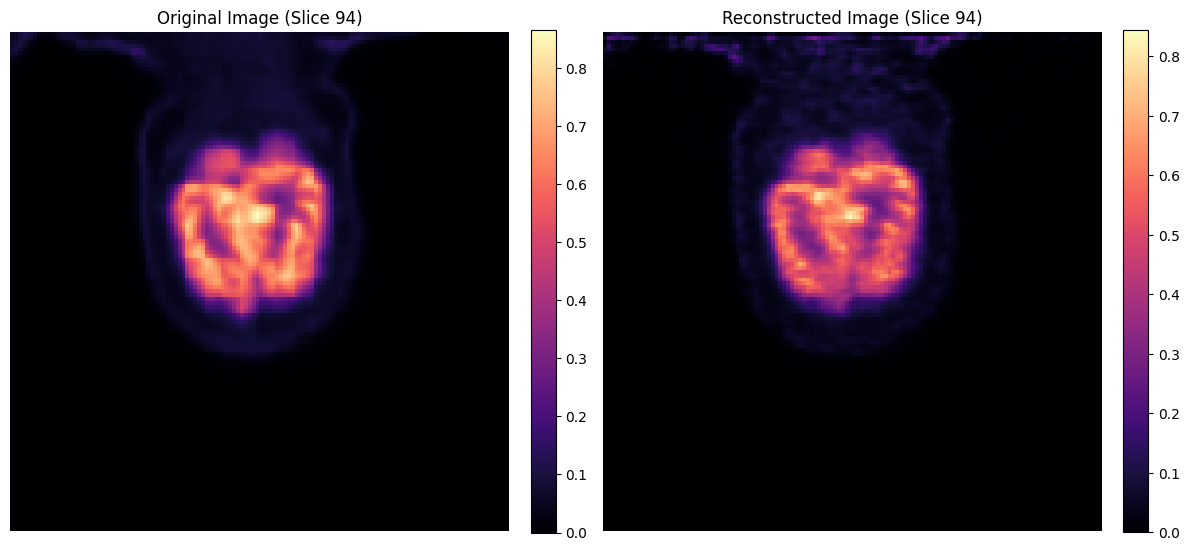
\includegraphics[width=0.98\textwidth]{Images/output}
    \vspace{-0.2cm}
    \caption{Comparison of original image and image reconstructed using the OSEM method}
    \vspace{-0.2cm}
    \label{fig:pet_reconstruction}
\end{figure*}

However, the standard MLEM algorithm converges slowly when processing large datasets. The Ordered Subset Expectation Maximization (OSEM) algorithm accelerates convergence by dividing the projection data into $S$ subsets $S_1,\dots,S_S$. In OSEM implementation, the measurement data $\{y_i\}_{i=1}^N$ is divided into $S$ subsets, each typically containing $N/S$ projection elements. Each update uses only one subset to update $\lambda_j$. A "complete OSEM iteration" is completed after cycling through all subsets.
Let $S_k$ represent the subset of projection indices used in the k-th iteration, then the OSEM update formula can be expressed as:
\begin{equation}
    \lambda_j^{(k+1)}
\;=\;
\lambda_j^{(k)}
\;\times\;
\frac{\displaystyle \sum_{i \in S_{k}} \frac{p_{ij}}{\sum_{\ell} p_{i\ell}\,\lambda_{\ell}^{(k)}} \; y_i}
{\displaystyle \sum_{i \in S_{k}} p_{ij}}
\end{equation}
By sequentially cycling through these subsets (e.g., using $S_1$ for the 1st iteration, $S_2$ for the 2nd, ..., $S_S$ for the S-th, then returning to $S_1$, and so on), the OSEM algorithm can approximate a complete MLEM update with fewer effective iterations, thus obtaining an image close to convergence in less time.

In modern PET software frameworks, the system matrix $p_{ij}$ is typically not stored as a large two-dimensional array, but is implicitly calculated through \textbf{projectors} and \textbf{backprojectors}. For each voxel j, the projector calculates its contribution to the measurement data $y_i$; the backprojector assigns the ratio of measured to expected data back to the voxel grid. This approach effectively reduces memory requirements when processing large volumes of data.

The algorithms described in this paper are based on the PyTomography library\cite{POLSON2025102020}. PyTomography is an open-source Python library for medical image reconstruction, providing a modular framework for system matrix construction, likelihood function computation, and reconstruction algorithm development. The library leverages PyTorch's GPU acceleration capabilities and the parallelproj library for efficient parallel computation. Its flexible modular design makes it easy to decouple system matrices, likelihood functions, and reconstruction algorithms, facilitating integration with various Python toolsets for new imaging modalities. Currently, the library has been successfully applied in fields such as parallel-hole SPECT and list-mode PET imaging, providing a highly optimized and user-friendly software platform for medical image reconstruction. We tested it using a brain PET dataset, and the comparison between the original image and the reconstructed image is shown in Figure~\ref{fig:pet_reconstruction}.


% \textbf{Initialization}: The image estimate $\lambda_j^{(0)}$ is typically initialized to a uniform value, or using a transmission image if available.
% \textbf{Regularization}: Pure OSEM algorithms may amplify noise, especially after multiple iterations. In practice, methods such as \textbf{post-smoothing} or \textbf{penalized likelihood} (adding spatial priors) are often used to control noise and obtain clearer images.
% \textbf{Termination criteria}: OSEM algorithms typically run for a fixed number of iterations, or until the change between updates is small enough.

% \subsection{Deep Learning for PET Reconstruction}


%!TEX root = ../Manual.tex
\section{Implementation Methods}
\label{chap:methods}


As shown in Figure \ref{fig:reconstruction_workflow}, this study proposes an innovative incomplete ring PET reconstruction framework that effectively addresses the data incompleteness problem caused by missing detectors through a multi-stage strategy. In the first stage, the system first processes incomplete sinograms (top left) resulting from missing detectors, completing the missing data through a trained optimized U-Net deep learning model to generate complete sinograms (top right). This sinogram restoration process fully utilizes the five-channel input strategy described in Chapter 3, effectively integrating spatial and temporal context information.

\begin{figure*}[ht]
    \centering
    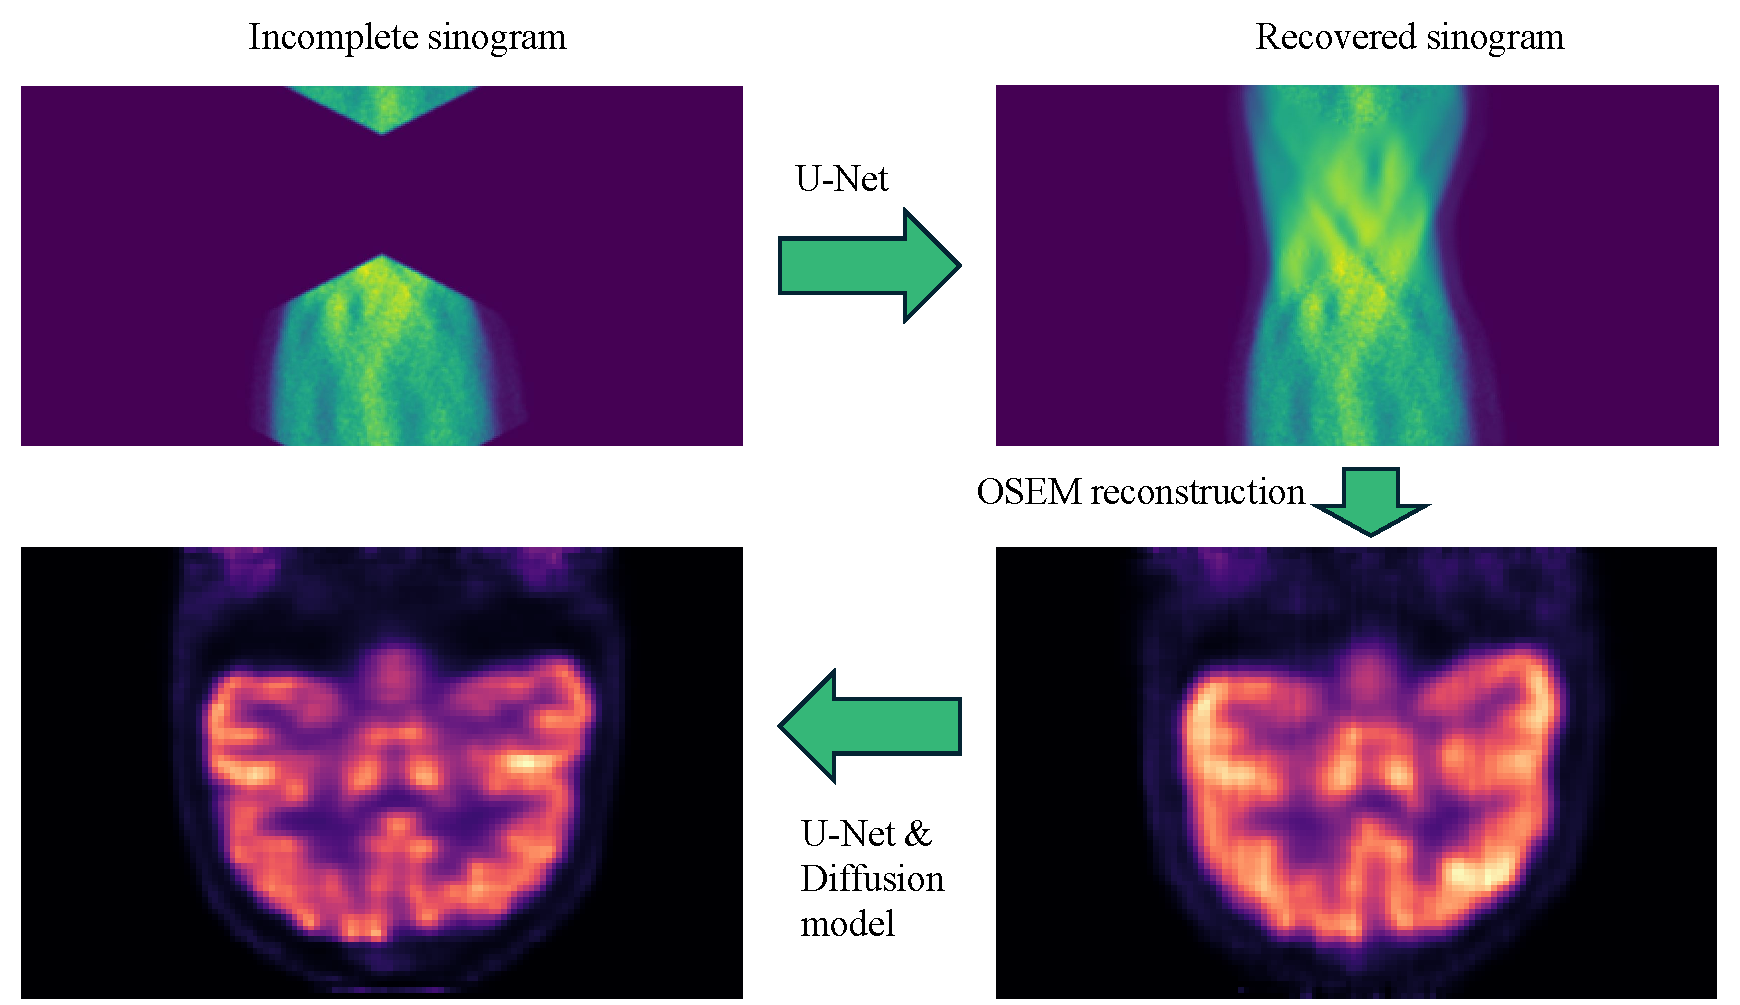
\includegraphics[width=\textwidth]{Images/reconstruction_workflow}
    \vspace{-.5cm}
    \caption{Overall flow diagram of the incomplete ring PET reconstruction method. First, incomplete sinograms due to missing detectors (top left) are repaired through a U-Net deep learning model to generate complete sinogram data (top right). Subsequently, the complete sinogram is converted into a PET image (bottom right) using the OSEM iterative reconstruction algorithm. For comparison, the bottom left image shows a PET image reconstructed directly from incomplete data using a coarse-to-fine framework (dual-model architecture with U-Net and diffusion model). This method effectively compensates for data loss caused by incomplete ring geometry, achieving high-quality brain PET image reconstruction that preserves key anatomical structures and tracer distribution features.}
    \vspace{-.2cm}
    \label{fig:reconstruction_workflow}
\end{figure*}

% \subsection{U-net Deep Learning Model}

\subsection{System Model and Data Simulation}
Assume a standard PET ring geometry with \(R\) axial rings, each containing \(D\) detectors, with each detector assigned a unique identification number used to precisely locate the photon pair's detection position when recording coincidence events. For example, consider a 42-ring system (i.e., \(R=42\)), with 182 detectors per ring, arranged in a cylindrical structure with radius \(\rho\). We map the 3D image grid (e.g., \(\text{size}=128\times128\times128\) voxels) to physical space by defining voxel dimensions, approximating the entire scanner geometry realistically. For instance, if the field of view diameter is 25 centimeters and the in-plane matrix size is 128, then each in-plane voxel size is:
\begin{equation}
\Delta x \approx \Delta y \approx \frac{25\,\text{cm}}{128} \approx 1.95\,\text{mm}.
\end{equation}
Axially, we can set \(\Delta z\) based on the typical axial coverage of a PET scanner. This high-precision spatial division ensures that the reconstructed images accurately reflect the anatomical structure of the scanned area.

The PET scanner used in this study employs a highly optimized detector system configuration, achieving comprehensive three-dimensional detection capabilities. The scanner's radius ($\rho$) is precisely set at 380.56 millimeters, achieving an optimal balance between spatial resolution and system sensitivity. The detector system adopts a multi-level organizational structure: at the microscopic level, crystal elements have lateral dimensions of 4.03125 millimeters and axial dimensions of 5.31556 millimeters, with this precise crystal size design ensuring high spatial resolution capability; at the macroscopic level, the detector construction includes 34 lateral sectors (rsectorTransNr) and a single axial sector arrangement (rsectorAxialNr). Each module is carefully designed to include 16 lateral (crystalTransNr) and 9 axial (crystalAxialNr) crystal elements, with the spacing between adjacent crystals (crystalTransSpacing and crystalAxialSpacing) optimized to achieve maximum detection efficiency. In the axial direction, the system has 4 modules (moduleAxialNr), maintaining a precise spacing of 50.64004 millimeters between modules (moduleAxialSpacing), a configuration that ensures detection sensitivity while maintaining an appropriate axial field of view range.
\begin{figure*}[htbp]
    \centering
    \vspace{-0.2cm}
    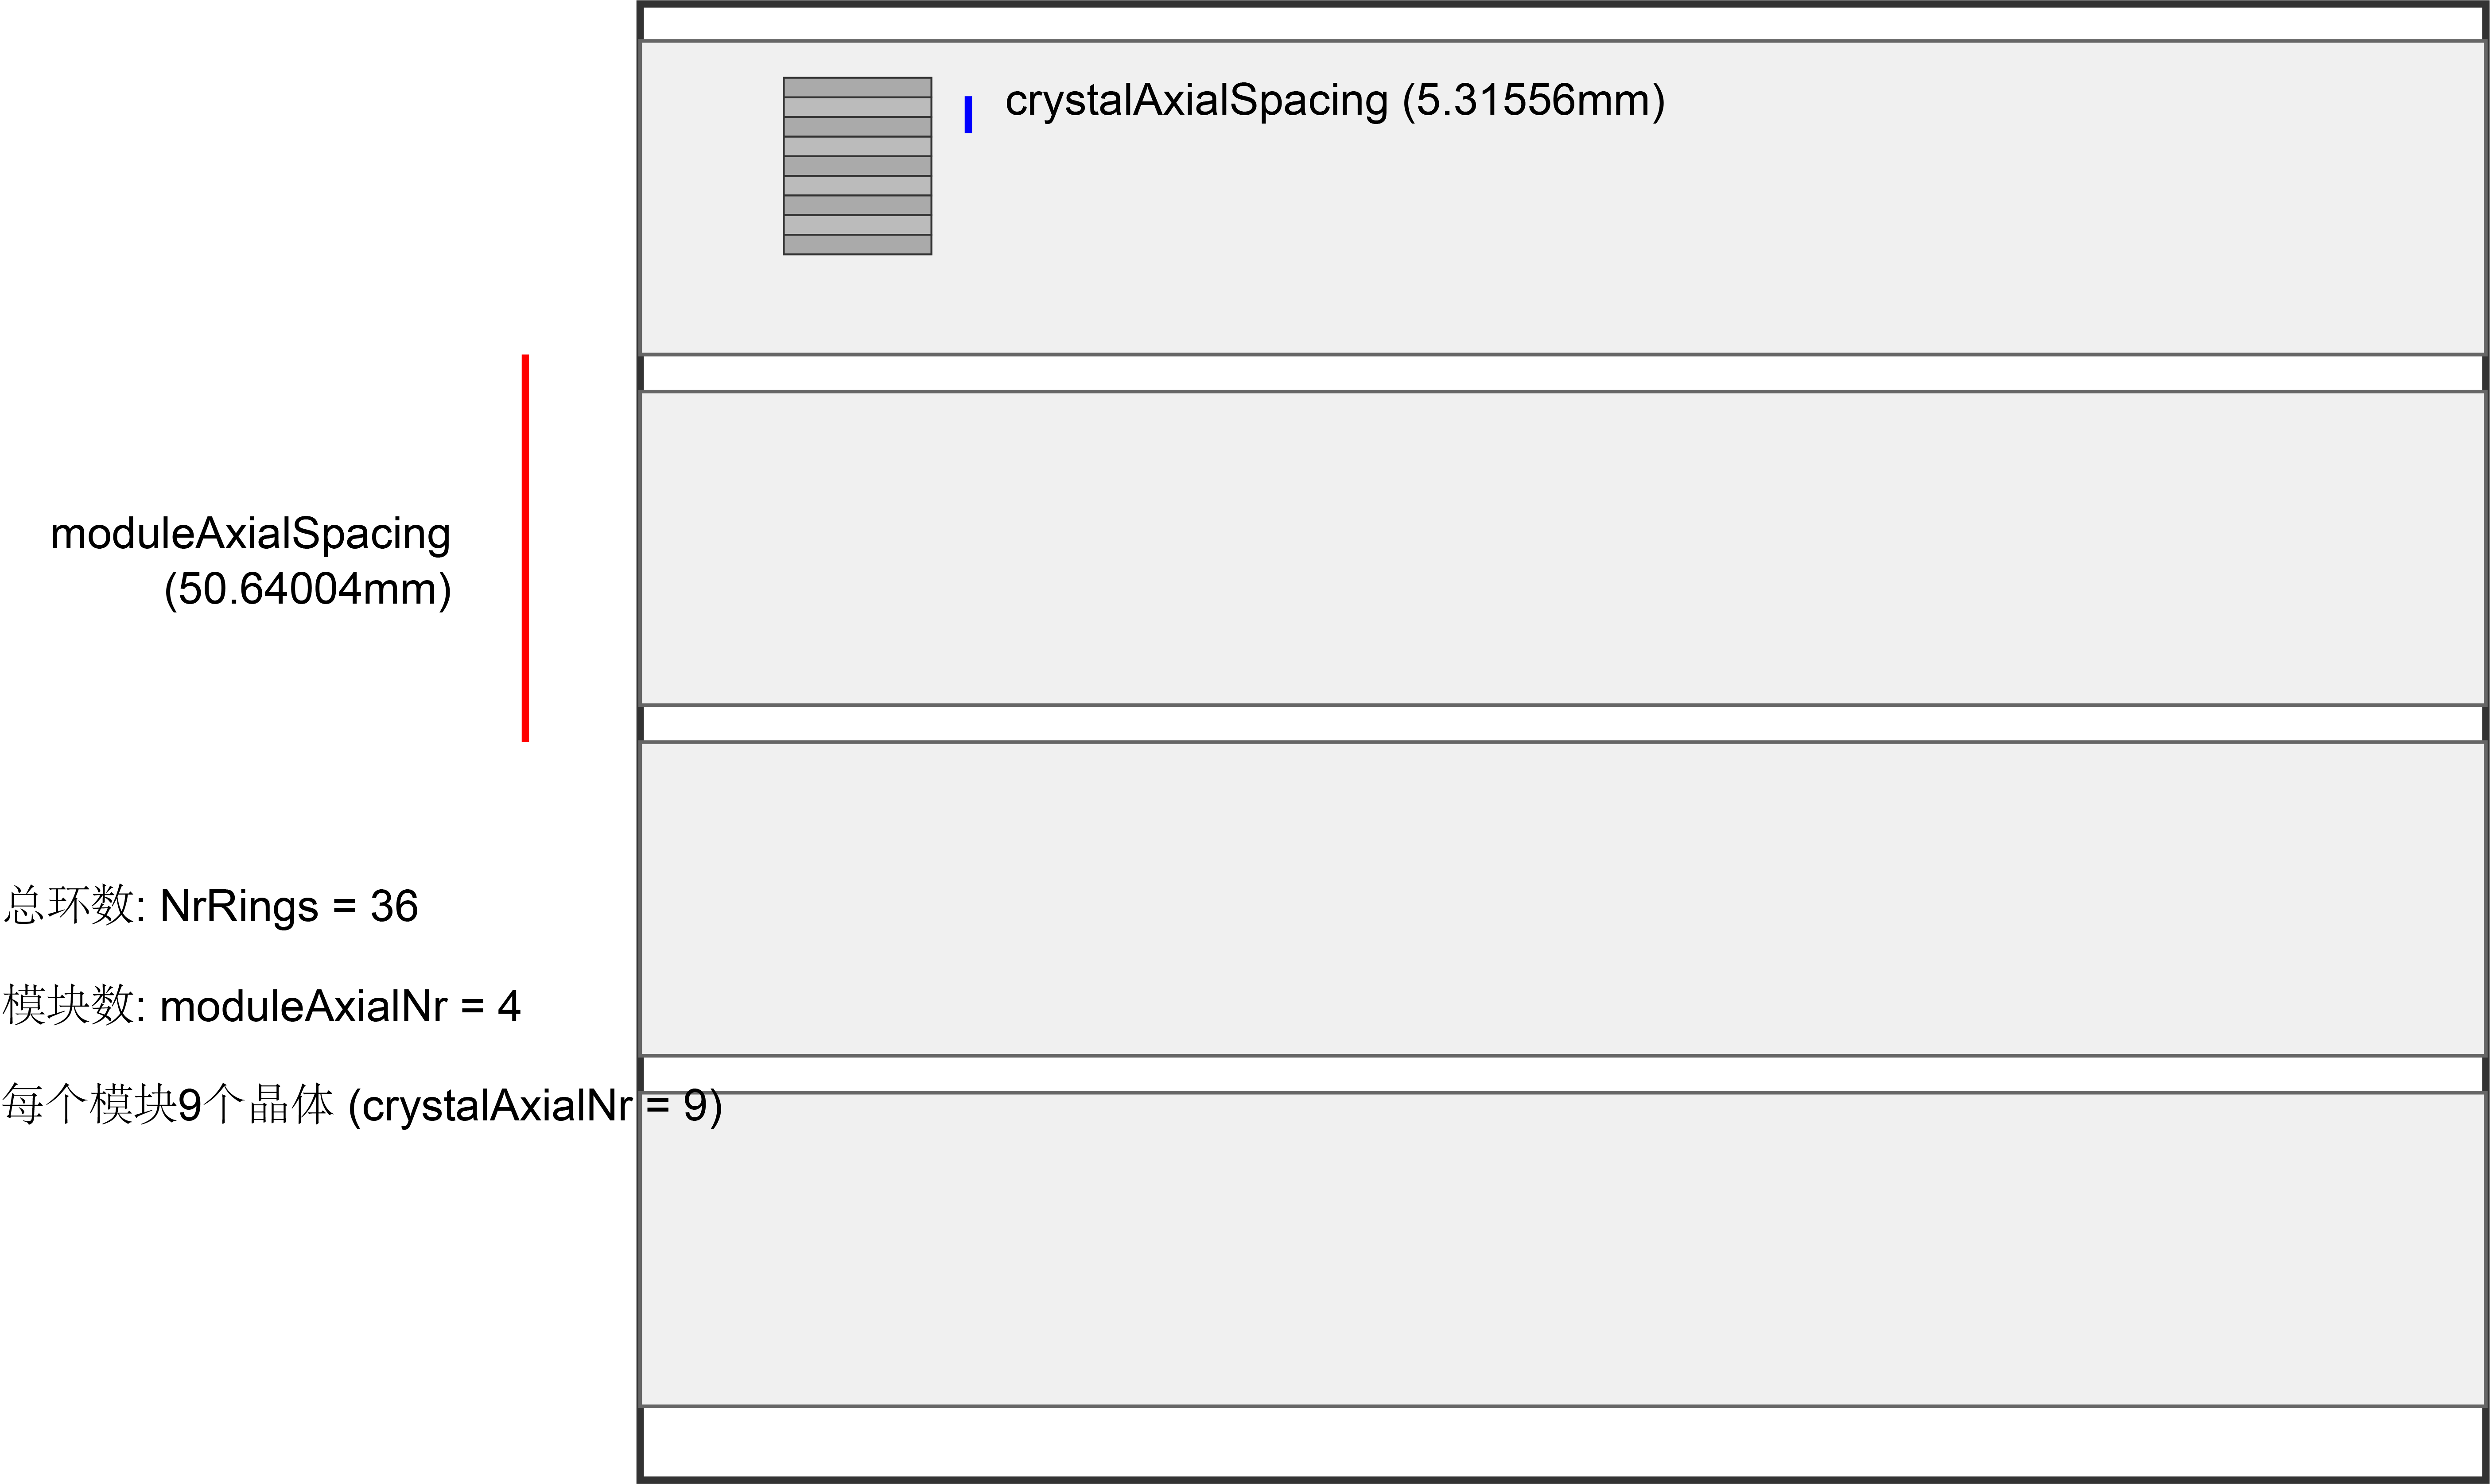
\includegraphics[width=0.7\textwidth]{Images/pet-side-view}
    \vspace{-0.2cm}
    \caption{Side view schematic of PET scanner detector structure.}
    \vspace{-0.2cm}
    \label{fig:pet_structures_side}
\end{figure*}
The system's data recording uses a list-mode format to record various coincidence events during the scanning process. The system supports time-of-flight (TOF) detection functionality, with 29 time bins (num\_tof\_bins), a full width at half maximum of the time resolution window (tof\_fwhm) of 57.71 millimeters, and a measurement range (tof\_range) reaching 735.7705 millimeters. However, due to current device performance limitations, this study could not fully utilize TOF technology to improve spatial resolution. Each event entry consists of three basic components, stored in tensor format. A typical list-mode event data structure is as follows:

\begin{verbatim}
[898, 3334, 11]
[816, 16375, 18]
[1073, 18816, 14]
[1529, 13781, 13]
[1537, 18663, 14]
\end{verbatim}

In this format, the first two numbers represent the identification numbers of the detector pair recording the coincidence event. The third number represents the time-of-flight information of the event, which, although not fully utilized in this study to enhance image quality, is retained for future data processing and analysis after system upgrades. To improve the system's sensitivity and accuracy, the detector system also includes submodule structures (submoduleAxialNr and submoduleTransNr both equal to 1), but in the current configuration, the submodule spacing (submoduleAxialSpacing and submoduleTransSpacing) is set to 0 to simplify system complexity.

In the current implementation process, due to the lack of MRI or CT data to obtain gamma ray absorption distribution maps, the system cannot use $\mu$ maps (linear attenuation maps) or component-based normalization files. This limitation means that the reconstruction process can only use list-mode data as input and cannot perform attenuation correction. When interpreting reconstruction results, this limitation's impact on image quality and quantitative accuracy must be considered.

\begin{figure*}[htbp]
\centering
\vspace{-0.2cm}
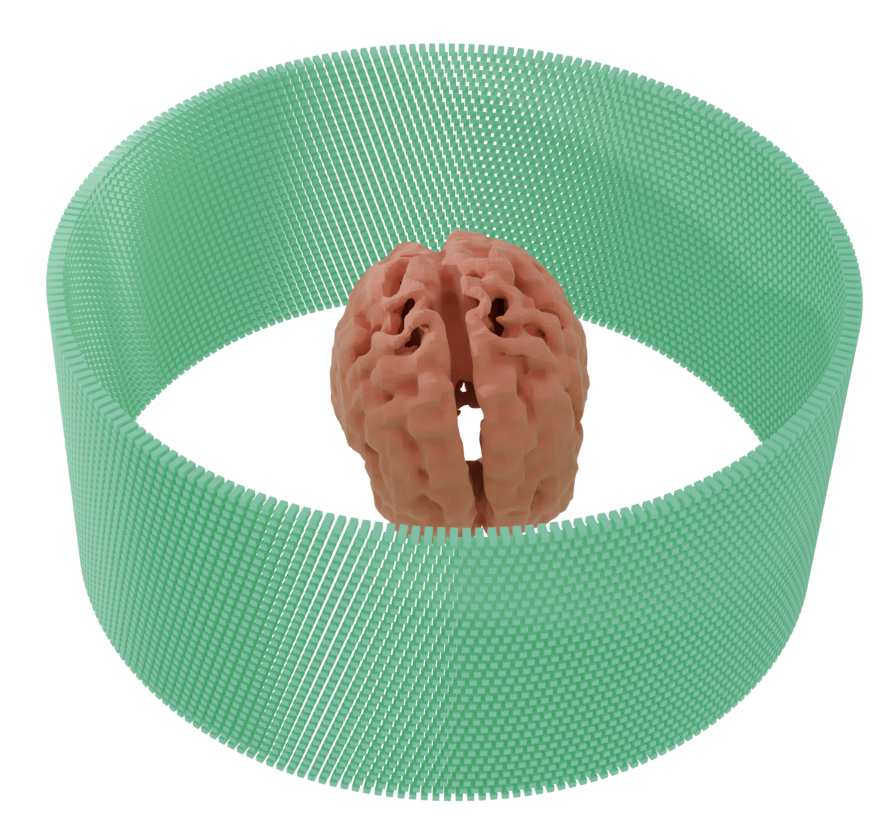
\includegraphics[width=0.45\textwidth]{Images/Thehumanbrainisnotmissing3}
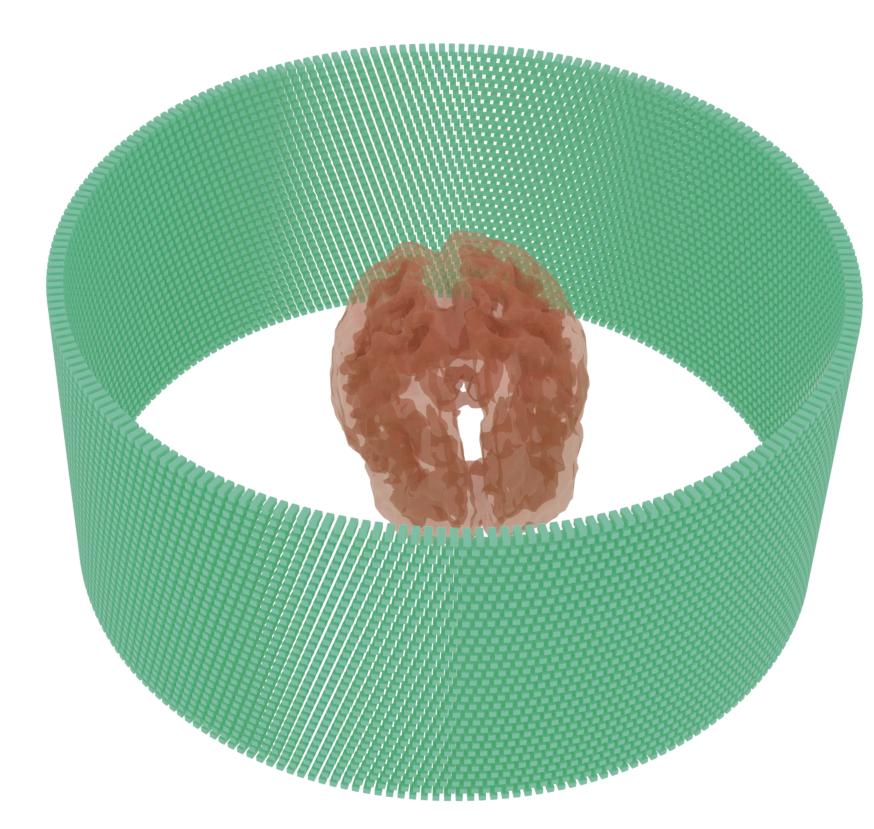
\includegraphics[width=0.45\textwidth]{Images/Thehumanbrainisnotmissing4}
\vspace{-0.2cm}
\caption{Three-dimensional schematic of PET scanner detector structure, with the right image showing a perspective view.}
\vspace{-0.2cm}
\label{fig:pet_structures}
\end{figure*}



We refer to the fully functional scenario where all \(R\) rings and all \(D\) detectors are working as the \emph{complete ring} configuration, as shown in Figure~\ref{fig:pet_structures}. The data simulation process is as follows:
\textbf{Starting with real 3D images.} We have high-resolution brain PET data or a synthetic phantom \(\mathbf{X}\in\mathbb{R}^{128\times128\times128}\).

\textbf{Randomly generating emission events.} We sample a specified number of emission events (e.g., 20 million) from the probability density function implied by \(\mathbf{X}\). Each voxel's value is interpreted as proportional to its tracer concentration probability.

\textbf{Simulating annihilation.} For each emission event, we assume it annihilates with an electron in the same voxel or nearby, producing two photons at 180\(^\circ\) opposite directions, each carrying 511 keV.

\textbf{Calculating detector hits.} Using geometric ray tracing, we calculate which detector pairs would detect these photons. This determines the LOR associated with each event, effectively generating a \emph{list-mode} dataset.

\textbf{Generating sinograms.} We can optionally sort the list-mode data into sinogram bins \(\mathbf{S}\) by radial, angular, and axial coordinates. This generates the standard 3D sinogram representation for PET.

Then, we use standard iterative reconstruction (e.g., OSEM) to reconstruct the baseline reconstruction volume \(\mathbf{Y}_A\) from \(\mathbf{S}\) (or directly from list-mode). This reconstruction from complete data is typically considered higher quality.
\begin{figure*}[htbp]
    \centering
    \vspace{-0.2cm}
    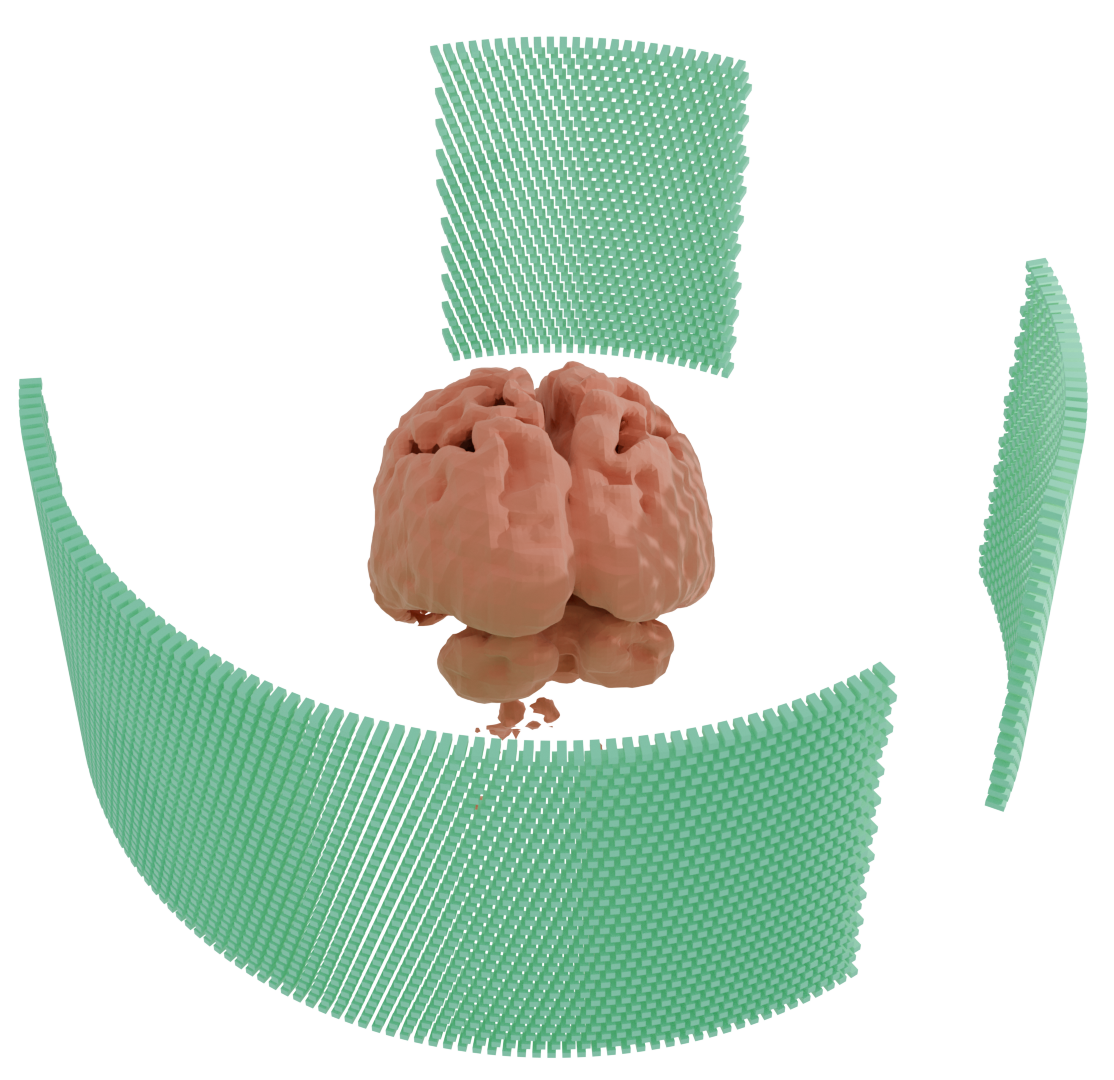
\includegraphics[width=0.45\textwidth]{Images/Thehumanbrainismissing5}
    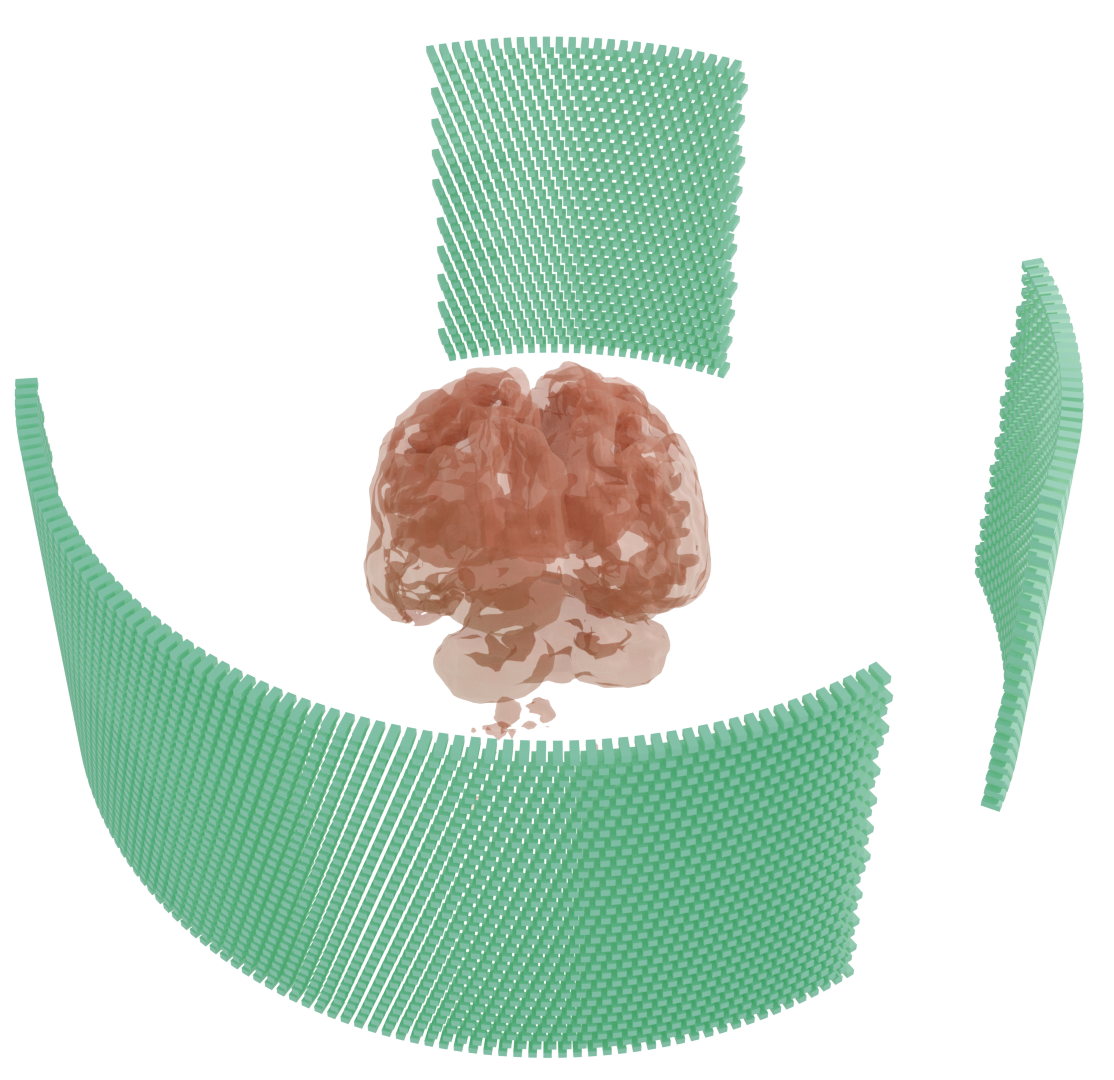
\includegraphics[width=0.45\textwidth]{Images/Thehumanbrainismissing4}
    \vspace{-0.2cm}
    \caption{Three-dimensional schematic of incomplete ring PET scanner detector structure, with the right image showing a perspective view.}
    \vspace{-0.2cm}
    \label{fig:pet_structures2}
\end{figure*}
In the \emph{incomplete ring} scenario, we remove parts of the detectors from the scanning geometry. The simplest approach is to remove all detectors from one or more complete rings, or remove angular segments from each ring. For example, suppose we remove one complete ring, so we're effectively only collecting data from \(R-1\) rings. The data simulation process is the same as the complete case, with the only difference being that events falling on the missing ring would not be recorded, as shown in Figure~\ref{fig:pet_structures2}.

Due to missing LORs, the incomplete data reconstructed image \(\mathbf{Y}_B\) typically has lower quality. In practice, we can reconstruct from the incomplete sinogram \(\mathbf{S}_{\text{incomplete}}\), i.e., \(\mathbf{Y}_B = \text{Reconstruct}(\mathbf{S}_{\text{incomplete}})\). This \(\mathbf{Y}_B\) can serve as input to our network, while \(\mathbf{Y}_A\) from complete data (same subject) can serve as the training target. The reconstruction from complete data \(\mathbf{Y}_A\) effectively represents the \emph{ground truth} of the tracer distribution for the same subject under ideal scanning conditions. In low-dose or incomplete coverage scenarios, the difference between \(\mathbf{Y}_B\) and \(\mathbf{Y}_A\) can be quite significant.

\subsection{Sinogram Reconstruction Based on Attention U-Net}

Although traditional U-Net performs excellently in medical image segmentation and reconstruction tasks, it lacks the ability to selectively focus on key features when dealing with complex incomplete ring PET sinogram restoration problems. The Attention U-Net adopted in this study enhances the model's perception of important feature regions through spatial attention mechanisms while suppressing the influence of irrelevant features, which is crucial for restoring sinograms from incomplete data.

The core innovation of Attention U-Net lies in the introduction of attention gating (AG) modules in the skip connection path of the standard U-Net, as shown in Figure 3.7. These AG modules can adaptively highlight significant structures in the feed-forward feature maps while suppressing irrelevant regions that might lead to prediction errors. For sinogram reconstruction tasks, this mechanism is particularly effective because it can selectively focus on structural features around missing areas, thereby more accurately inferring missing angular data. The mathematical expression of attention gating can be formalized as:

\begin{equation}
\alpha_i^l = \sigma_2(\psi^T(\sigma_1(W_x^T x_i^l + W_g^T g_i + b_g)) + b_\psi)
\end{equation}

where $x_i^l$ is the low-level feature from the encoder, $g_i$ is the gating signal from the decoder (high-level feature), $\sigma_1$ and $\sigma_2$ are ReLU and Sigmoid activation functions respectively, and $W_x$, $W_g$, $b_g$, and $b_\psi$ are learnable parameters. $\alpha_i^l \in [0,1]$ is the calculated attention coefficient used to control the importance of features.

After processing through the attention gate, the features can be represented as:

\begin{equation}
\hat{x}_i^l = x_i^l \cdot \alpha_i^l
\end{equation}

This mechanism allows Attention U-Net to adaptively focus on important image regions while maintaining the advantages of the original U-Net's encoder-decoder structure, particularly in cases of severe angular loss, with a stronger perception of sinogram continuity and consistency.
\begin{figure*}[htbp]
    \centering
    \vspace{-.2cm}
    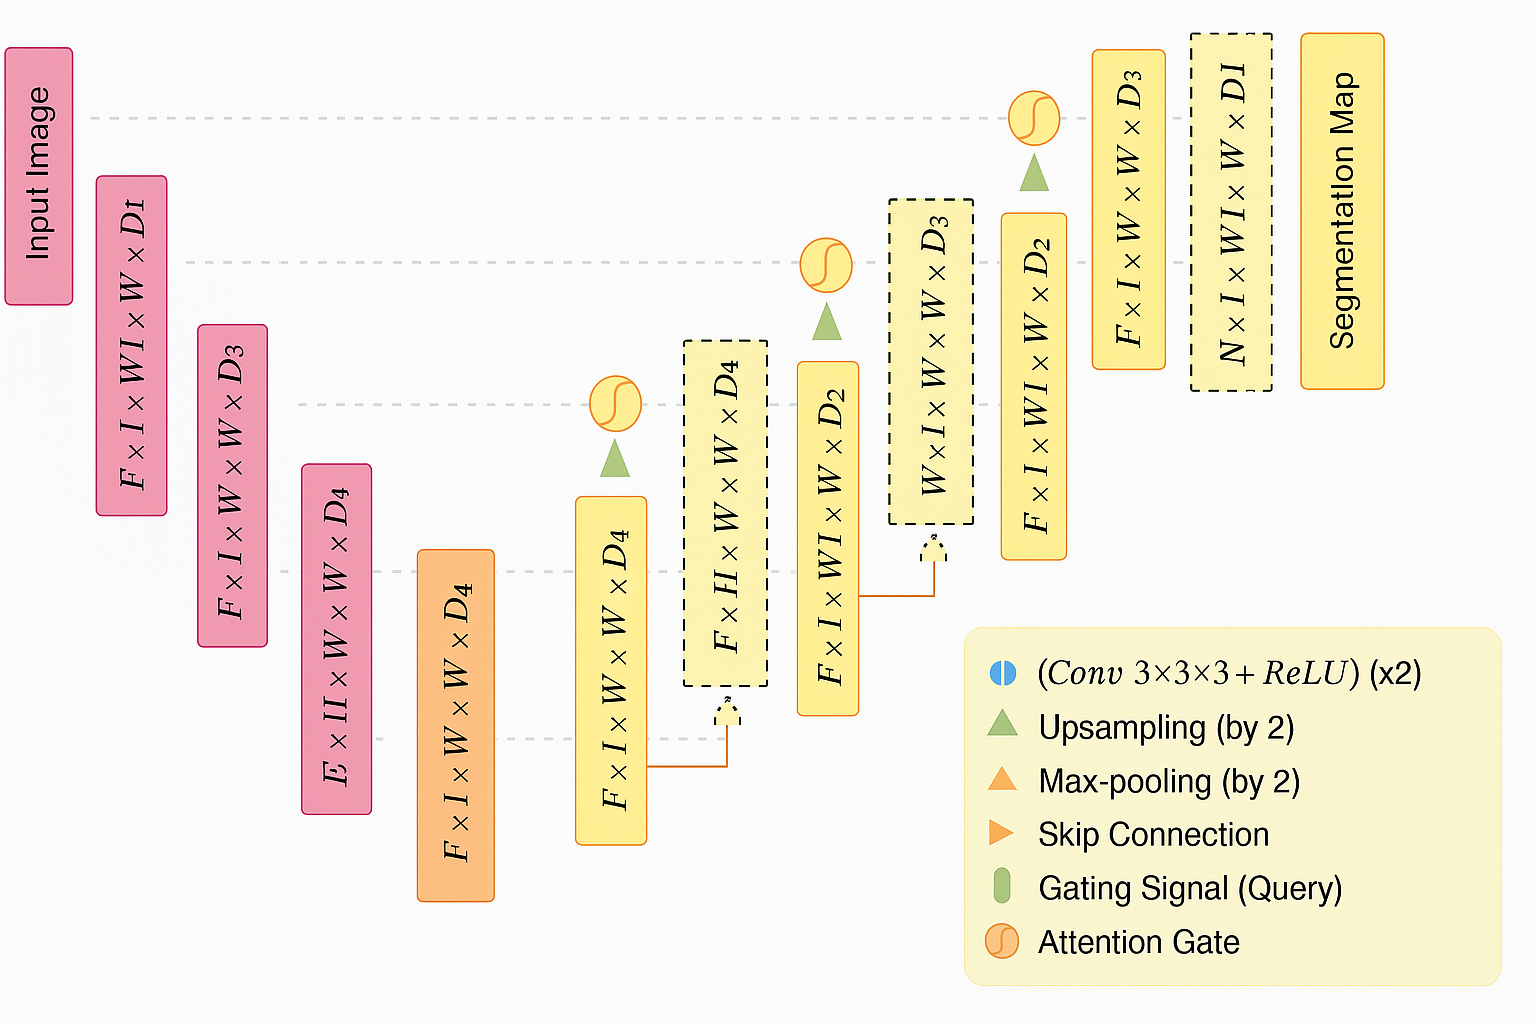
\includegraphics[width=0.8\textwidth]{Images/Unet.png}
    \vspace{-.3cm}
    \caption{Attention U-Net architecture diagram, showing how the attention gating mechanism enhances skip connection features.}
    \label{fig:unet_structure}
\end{figure*}
In the experimental implementation, we integrated AG modules into the skip connection path at each decoding stage, using $1\times1$ convolution to reduce channel dimensions, followed by applying attention coefficients for feature selection. This design enables the model to more precisely restore missing data when processing incomplete sinograms containing large-scale angular losses, while maintaining overall structural consistency and accurate signal distribution.

Experimental results show that compared to standard U-Net, Attention U-Net achieved significant improvements in sinogram reconstruction tasks, with an average increase of 1.24dB in PSNR metrics and 0.052 in SSIM metrics, validating the effectiveness of the attention mechanism in processing incomplete ring PET data.

Sinogram repair plays a crucial role in incomplete ring PET imaging, with its quality directly affecting the precision of reconstructed images. The training dataset used in this study consists of multidimensional tensors that effectively capture spatial and temporal context information, essential for accurate sinogram restoration. Each sinogram slice is expanded into a five-channel tensor, systematically integrating slices from spatial and temporal neighborhoods. As shown in Figure~\ref{fig:sinogram_structure}, the central channel of each input tensor corresponds to the current sinogram slice, while the direct spatial neighbors (slices $j-1$ and $j+1$) and temporal neighbors from previous and subsequent sinogram periods (slices $j-N_2$ and $j+N_2$) constitute the other four channels. These neighboring slices are crucial for enriching the model's understanding of local structural continuity and temporal consistency.

\begin{figure*}[htbp]
\centering
\vspace{-.3cm}
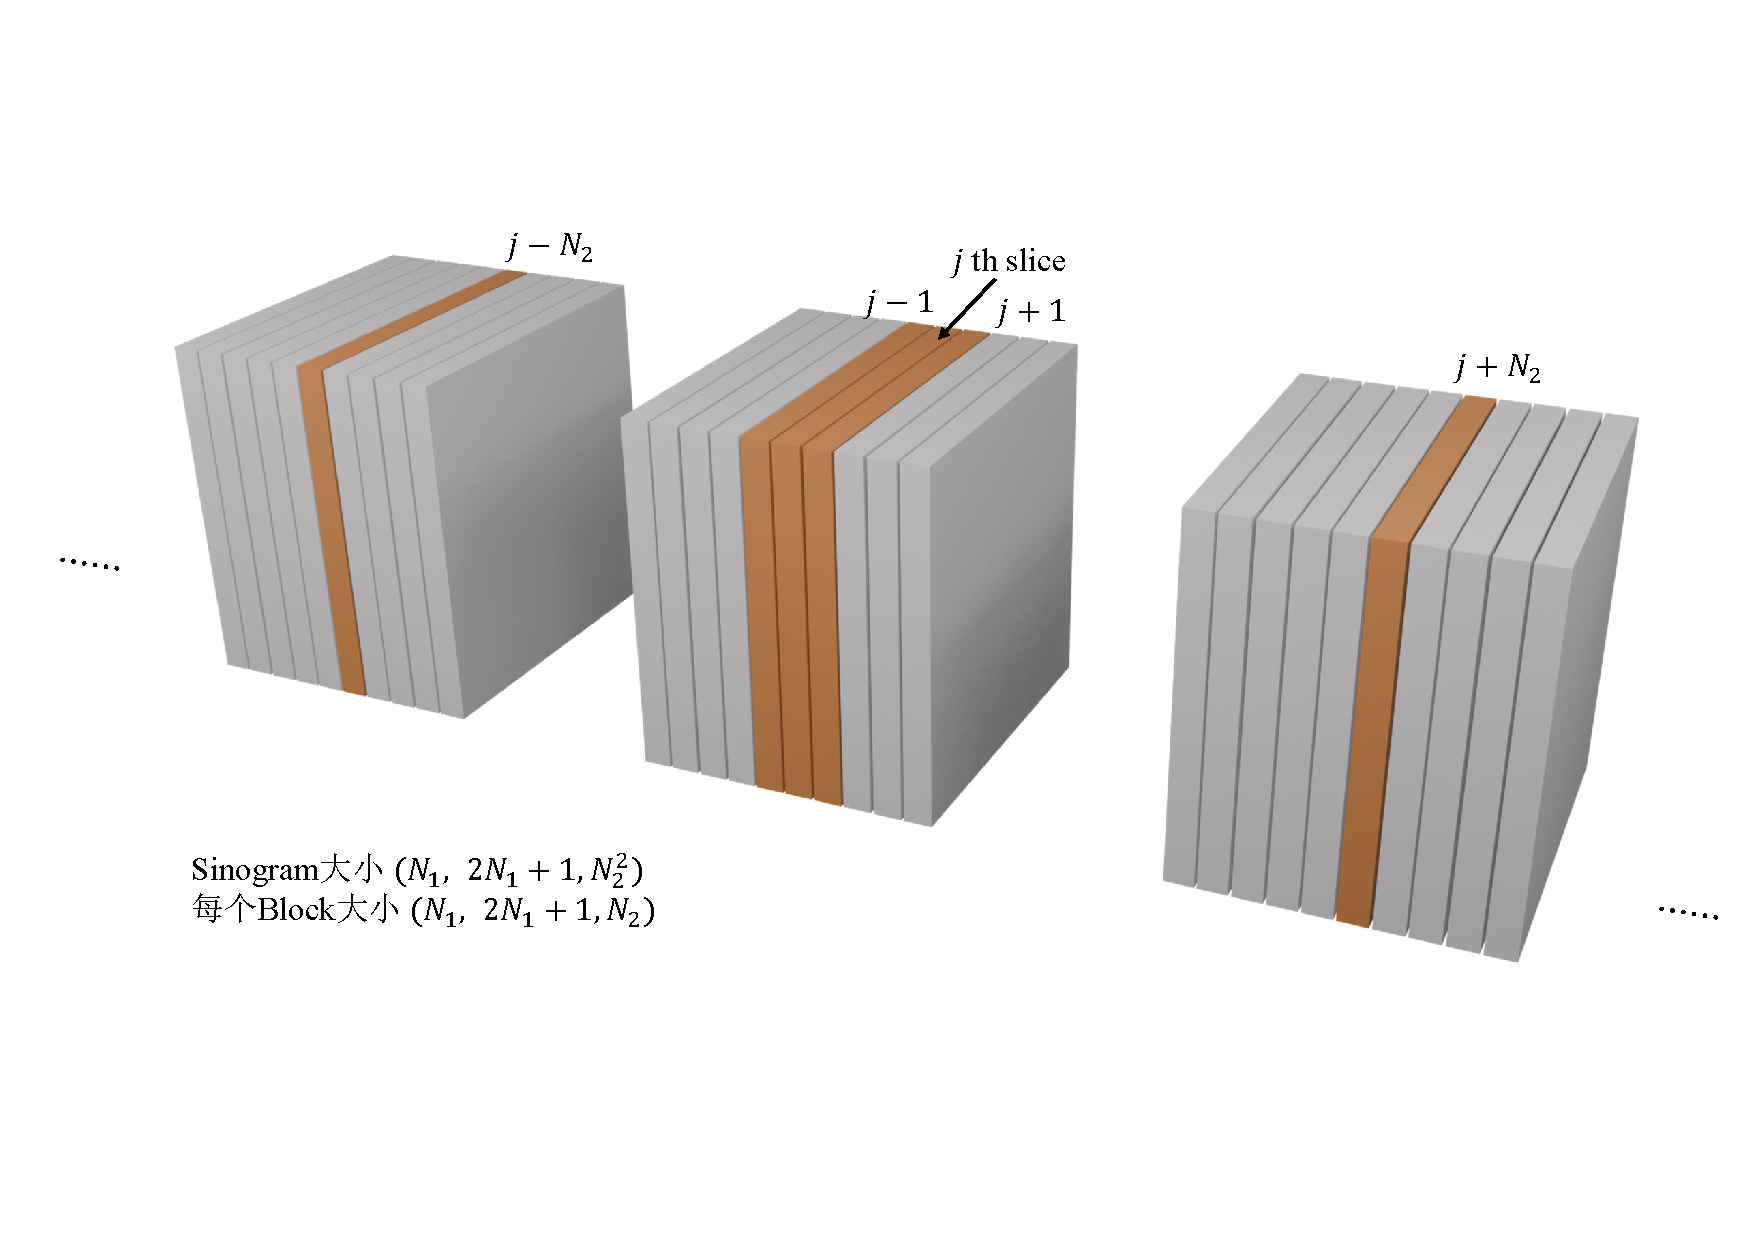
\includegraphics[width=0.96\textwidth]{Images/fdafads.pdf}
\vspace{-.3cm}
\caption{Visualization of the five-channel tensor preparation of sinogram data for training. Each cube represents a sinogram slice block with dimensions $(N_1, 2N_1+1, N_2)$. The orange highlighted parts are the selected slices ($j-N_2, j-1, j, j+1, j+N_2$), which form the five-channel input for the restoration model, showing the spatial and temporal relationships captured in each input tensor.}
\label{fig:sinogram_structure}
\end{figure*}


In this study, a five-channel input tensor is used to construct training data. For each central slice $j$, a multidimensional feature is built by fusing its spatial adjacent slices ($j-1$ and $j+1$) with temporal adjacent slices ($j-42$ and $j+42$). Boundary handling adopts a mirror padding strategy: when adjacent indices exceed the dataset range, the central slice itself is used for channel filling, ensuring input dimension consistency. Finally, each training sample forms a $5\times H\times W$ tensor, effectively integrating spatiotemporal neighborhood information.\par

The network architecture adopts an improved U-Net model (see Table\ref{tab:unet_architecture}), with an encoder-decoder structure including convolution, pooling, upsampling, and skip connection modules. The encoder part uses $3\times3$ convolution kernels with batch normalization and ReLU activation functions, implementing feature dimensionality reduction through max pooling; the decoder uses transposed convolution/bilinear interpolation for resolution recovery, and shallow detail features are fused through skip connections. The bottleneck layer achieves high-level semantic representation through 1024-dimensional features.



Model training uses the Adam optimizer with an initial learning rate of $10^{-4}$ and introduces $10^{-5}$ weight decay to prevent overfitting. Training efficiency is enhanced through mixed precision computation and gradient scaling techniques, combined with a ReduceLROnPlateau dynamic learning rate scheduler (with a decay factor of 0.3 when validation loss shows no improvement for 3 consecutive epochs), achieving stable convergence.


On the validation set, the model achieved excellent performance with MSE=0.301745, PSNR=35.6421 dB, and SSIM=0.9588. The PSNR value indicates high fidelity of the reconstructed signal, while the SSIM metric validates the preservation of structural features. Experimental results show that the multi-channel U-Net method proposed in this paper can effectively improve sinogram repair quality, providing a reliable foundation for subsequent CT image reconstruction. This method significantly improves the limitations of traditional single-channel models by fusing spatiotemporal context information, offering a new technical approach for the medical imaging processing field.




\subsection{Diffusion Probabilistic Models}
Diffusion probabilistic models (DPMs) have attracted great attention in image synthesis and inverse problems for their ability to produce state-of-the-art results and training stability. Unlike GANs that rely on adversarial objectives, DPMs are trained by maximizing a variational lower bound on the data log-likelihood. This chapter covers the core principles and mathematical formulations of denoising diffusion probabilistic models relevant to the proposed method.
Diffusion models are a class of probabilistic generative models proposed by \textit{Sohl-Dickstein et al.}\cite{pmlr-v37-sohl-dickstein15}, and later widely applied in image generation tasks by \textit{Ho et al.}\cite{ho2020denoisingdiffusionprobabilisticmodels}. The basic idea is to gradually inject noise into the data distribution, transforming it into an isotropic Gaussian distribution. In the generation stage, the target data distribution is gradually restored from pure noise through a learned reverse denoising process. This framework can be divided into two main stages:
\textbf{Forward Process}: Gradually adding noise to the data, making the data distribution approach a Gaussian distribution;
\textbf{Reverse Process}: Starting from Gaussian noise, gradually denoising to generate samples consistent with the original data.
Diffusion models have achieved significant results in image, speech, text, and other fields, with their stability and generation quality attracting widespread attention.

\subsubsection{Forward Process}
The forward process gradually adds noise to the data $\mathbf{x}_0 \in \mathbb{R}^d$ through a Markov chain, mathematically expressed as:
\begin{equation}
    q(\mathbf{x}_{1:T} \mid \mathbf{x}_0) = \prod_{t=1}^T q(\mathbf{x}_t \mid \mathbf{x}_{t-1}),
\end{equation}
where each step's conditional probability is defined as:
\begin{equation}
    q(\mathbf{x}_t \mid \mathbf{x}_{t-1}) = \mathcal{N}(\mathbf{x}_t; \sqrt{1 - \beta_t} \mathbf{x}_{t-1}, \beta_t \mathbf{I}).
\end{equation}
Here, $\beta_t \in (0, 1)$ represents the noise intensity, a predetermined hyperparameter controlling the amount of noise added in each step.
Since the noise added at each step is a linear combination of Gaussian distributions, $\mathbf{x}_t$ can be directly calculated from $\mathbf{x}_0$. Using the properties of Gaussian distributions, we have:
\begin{equation}
    q(\mathbf{x}_t \mid \mathbf{x}_0) = \mathcal{N}(\mathbf{x}_t; \sqrt{\bar{\alpha}_t} \mathbf{x}_0, (1 - \bar{\alpha}_t) \mathbf{I}),
\end{equation}
where the cumulative coefficient $\bar{\alpha}_t$ is defined as:
\begin{equation}
    \bar{\alpha}_t = \prod_{s=1}^t \alpha_s, \quad \alpha_t = 1 - \beta_t
\end{equation}
This closed-form solution allows us to directly sample $\mathbf{x}_t$ from $\mathbf{x}_0$, greatly simplifying the derivation process during training.

\subsubsection{Reverse Process}
The reverse process aims to rebuild data starting from pure Gaussian noise through gradual denoising. Assuming the Markovian property of the forward process holds, the reverse process can also be represented by a Markov chain:
\begin{equation}
    p_\theta(\mathbf{x}_{0:T}) = p(\mathbf{x}_T) \prod_{t=1}^T p_\theta(\mathbf{x}_{t-1} \mid \mathbf{x}_t),
\end{equation}
where $p(\mathbf{x}_T)$ is a standard Gaussian distribution, and $p_\theta(\mathbf{x}_{t-1} \mid \mathbf{x}_t)$ represents the reverse conditional distribution. We typically assume it takes the form of a Gaussian distribution:
\begin{equation}
    p_\theta(\mathbf{x}_{t-1} \mid \mathbf{x}_t) = \mathcal{N}(\mathbf{x}_{t-1}; \boldsymbol{\mu}_\theta(\mathbf{x}_t, t), \sigma_t^2 \mathbf{I}).
\end{equation}
Here, the mean $\boldsymbol{\mu}_\theta$ and variance $\sigma_t^2$ are modeled by neural networks. To simplify implementation, $\sigma_t^2$ is often fixed as a constant.

\subsubsection{Model Training}

In practice, directly predicting $\mathbf{x}_{t-1}$ can be overly complex. We can simplify this problem by predicting the noise $\boldsymbol{\epsilon}$ in the forward process. According to the closed-form solution of the forward process:
\begin{equation}
    \mathbf{x}_t = \sqrt{\bar{\alpha}_t} \mathbf{x}_0 + \sqrt{1 - \bar{\alpha}_t} \boldsymbol{\epsilon}, \quad \boldsymbol{\epsilon} \sim \mathcal{N}(\mathbf{0}, \mathbf{I}),
\end{equation}
the model's task can be transformed into learning to predict the noise $\boldsymbol{\epsilon}$, i.e., approximating the true noise through a neural network $\boldsymbol{\epsilon}_\theta(\mathbf{x}_t, t)$.
For this purpose, the training objective is defined as minimizing the following mean squared error (MSE) loss:
\begin{equation}
    L_{\text{simple}}(\theta) = \mathbb{E}_{\mathbf{x}_0, \boldsymbol{\epsilon}, t}\bigl[\|\boldsymbol{\epsilon} - \boldsymbol{\epsilon}_\theta(\mathbf{x}_t, t)\|^2\bigr]
\end{equation}
This approach is not only simple but has also shown good performance in generation tasks.


The model's training objective is based on the variational lower bound (VLB), optimizing the generation process by maximizing the data likelihood $\log p_\theta(\mathbf{x}_0)$. Its bound form is:
\begin{equation}
    -\log p_\theta(\mathbf{x}_0) \leq \text{KL}\bigl(q(\mathbf{x}_T \mid \mathbf{x}_0) \| p(\mathbf{x}_T)\bigr) + \sum_{t=2}^T \text{KL}\bigl(q(\mathbf{x}_{t-1} \mid \mathbf{x}_t, \mathbf{x}_0) \| p_\theta(\mathbf{x}_{t-1} \mid \mathbf{x}_t)\bigr) - \log p_\theta(\mathbf{x}_0 \mid \mathbf{x}_1)
\end{equation}
In practice, directly optimizing this objective is relatively complex, and the simplified noise prediction loss $L_{\text{simple}}(\theta)$ is typically used for optimization, with the core being to learn the denoising process.

\subsubsection{Sampling}
In the generation stage, starting from Gaussian noise $\mathbf{x}_T \sim \mathcal{N}(\mathbf{0}, \mathbf{I})$, samples are gradually generated through the following formula:
\begin{equation}
    \mathbf{x}_{t-1} = \frac{1}{\sqrt{\alpha_t}} \bigl(\mathbf{x}_t - \frac{1 - \alpha_t}{\sqrt{1 - \bar{\alpha}_t}} \boldsymbol{\epsilon}_\theta(\mathbf{x}_t, t)\bigr) + \sigma_t \mathbf{z}, \quad \mathbf{z} \sim \mathcal{N}(\mathbf{0}, \mathbf{I})
\end{equation}
Here, $\sigma_t$ represents the noise intensity at each step.
Through multiple iterations, the finally generated $\mathbf{x}_0$ should approach the target data distribution.

% \subsection{Summary}
Diffusion models, as a generative modeling method combining the advantages of probabilistic graphical models and deep learning, achieve efficient generation through forward noise addition and reverse denoising processes, showing broad application prospects in fields such as image generation, speech synthesis, and text generation. In the inverse problem of PET reconstruction under incomplete ring conditions, the advantages of diffusion models are particularly prominent: they not only effectively avoid the mode collapse problem common in GANs, ensuring robust coverage of possible solutions, but can also effectively integrate learned priors for PET images, which is extremely important when large segments of sinogram data are missing; meanwhile, their iterative refinement characteristic highly aligns with the iterative image reconstruction methods (such as MLEM) widely used in the PET field. However, direct application of DPMs for reconstruction has issues of slow computation speed and insufficient consideration of partial data scale. To address these limitations, we propose an innovative coarse-to-fine method, effectively overcoming these challenges by introducing a deterministic, high-capacity coarse prediction module combined with a small-scale iterative diffusion model focused on residual reconstruction.



\subsection{Coarse-to-Fine Reconstruction Framework}

In this section, we outline the main workflow of the coarse-to-fine approach for reconstructing PET data from incomplete ring scanners. First, we introduce the system modeling description (i.e., how to simulate or process incomplete rings). Then, we detail the data generation steps for complete and incomplete rings, ultimately building our \emph{CPM + IRM} reconstruction architecture. Finally, we discuss the \emph{auxiliary guidance} and \emph{contrastive diffusion} strategies.





\subsubsection{Overall Coarse-to-Fine Framework}
\label{sec:overall_coarse_fine}
Applying diffusion probabilistic models directly to incomplete ring reconstruction typically faces the problem of high computational cost, as each inference requires multiple iterative steps. Additionally, for large 3D volumes (128\(^3\) or higher), pure diffusion methods may be challenging in terms of memory. Therefore, we adopt a \emph{coarse-to-fine} approach, where the \textbf{Coarse Prediction Module (CPM)} outputs an initial deterministic reconstruction from partial or degraded input, as shown in Figure~\ref{fig:coarse_to_fine_framework}. The
\textbf{Iterative Refinement Module (IRM)} implements a conditional diffusion process to estimate the residual \(\mathbf{r}_0\) between the coarse prediction and the ground truth.

\begin{figure*}[ht]
    \centering
    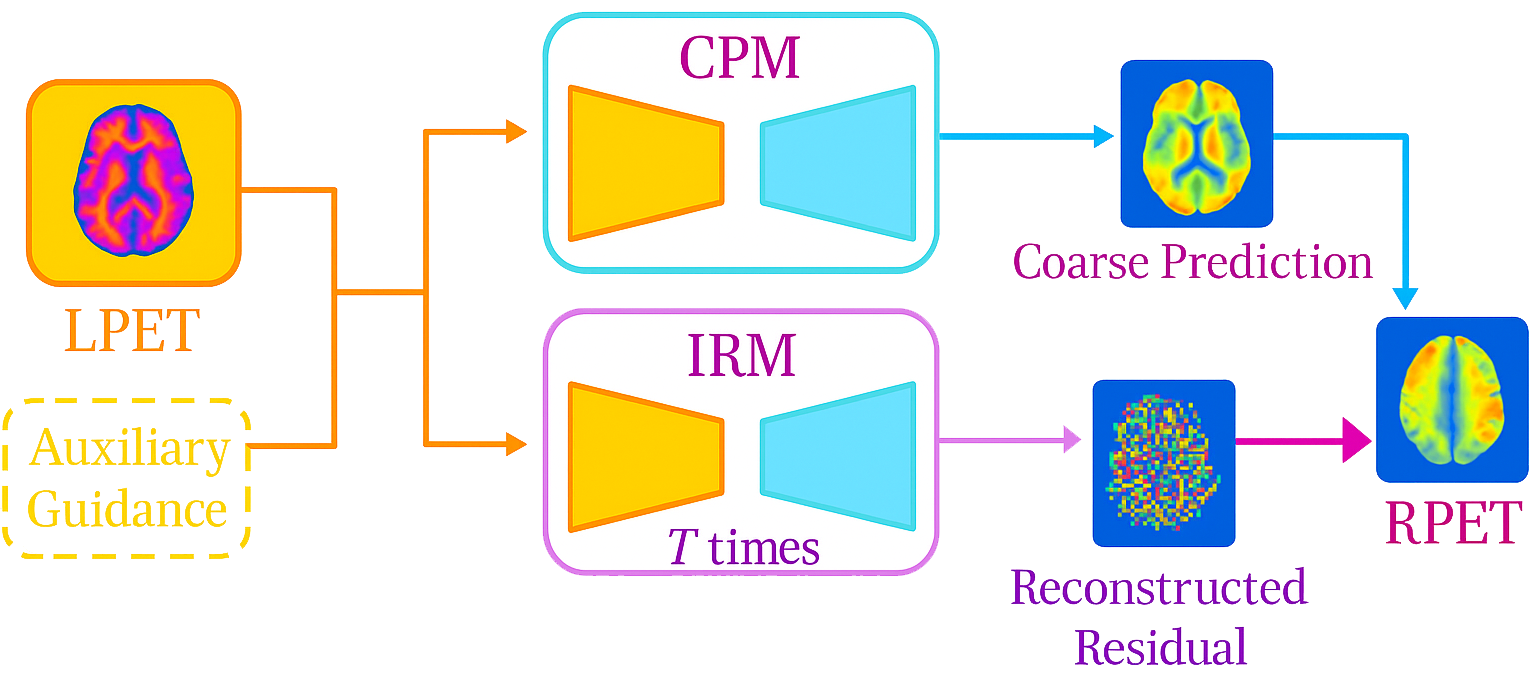
\includegraphics[width=0.8\textwidth]{Images/C2F.png}
    \caption{Overview of the coarse-to-fine incomplete ring PET reconstruction framework. The method contains two key modules: the Coarse Prediction Module (CPM) and the Iterative Refinement Module (IRM). The system first receives low-quality PET images (LPET) and auxiliary guidance information as input. The CPM generates preliminary reconstruction results (coarse prediction) through a single forward pass. Subsequently, the IRM, based on diffusion probabilistic models, reconstructs the residual signal through T iterative steps. Finally, the system combines the coarse prediction with the reconstructed residual to generate a high-quality refined PET image (RPET). This dual-stage design effectively balances computational efficiency with reconstruction quality, overcoming the limitations of traditional diffusion models in terms of computational cost.}
    \label{fig:coarse_to_fine_framework}
\end{figure*}


\subsubsection{Coarse Prediction Module (CPM)}
Let \(\mathbf{c}\) be our condition, including \(\mathbf{Y}_B\), the reconstructed PET image from incomplete data; \(\mathbf{X}_{\text{aux}}\), additional auxiliary guidance, such as adjacent slices or spectral transforms.



The CPM, denoted as \(P_\theta(\mathbf{c})\), is a deterministic deep network designed to generate a coarse reconstruction \(\mathbf{x}_\text{cp}\). This step effectively transfers most of the parametric complexity into a single forward pass. In practice, the CPM can be a relatively large U-net or other suitable backbone network, trained as follows:
\begin{equation}
\mathcal{L}_{\text{CPM}} = \|\mathbf{x}_\text{cp} - \mathbf{Y}_A\|_1,
\end{equation}
or using a mean squared error (MSE) loss. In our final method, we integrate the training of the CPM with the IRM into a single framework.

\subsubsection{Iterative Refinement Module (IRM)}
Once we have \(\mathbf{x}_\text{cp}\), we define \(\mathbf{r}_0 = \mathbf{Y}_A - \mathbf{x}_\text{cp}\) as the residual. Our goal is to learn a diffusion process to model:
\begin{equation}
p_\theta(\mathbf{r}_{t-1} \mid \mathbf{r}_t, \mathbf{c}) \approx q(\mathbf{r}_{t-1} \mid \mathbf{r}_t, \mathbf{r}_0),
\end{equation}
such that sampling from the IRM can yield a residual estimate \(\widehat{\mathbf{r}_0}\) from a random noise initialization. We can then reconstruct:
\begin{equation}
\widehat{\mathbf{Y}_A} = \mathbf{x}_\text{cp} + \widehat{\mathbf{r}_0}.
\end{equation}
Since the IRM focuses only on the residual, its capacity can be smaller. Moreover, the gap between \(\mathbf{x}_\text{cp}\) and \(\mathbf{Y}_A\) is typically significantly smaller than the gap between a random noise distribution and \(\mathbf{Y}_A\). This achieves faster convergence and fewer sampling time steps in practice.

\subsubsection{Training Objectives}
We follow the typical DPM training approach but treat \(\mathbf{y}_0=\mathbf{r}_0\) as the \emph{target data} in the diffusion sense. We combine the losses for CPM and IRM:
\begin{equation}
\mathcal{L}_{\text{main}} = \mathbb{E}_{(\mathbf{c},\mathbf{Y}_A)}\Big[
\underbrace{\|\mathbf{r}_0 - D_\theta(\mathbf{c},\mathbf{r}_t,t)\|_1}_{\text{IRM-latent}}\Big] 
\quad \text{where} \quad \mathbf{r}_t=\sqrt{\gamma_t}\,\mathbf{r}_0 + \sqrt{1-\gamma_t}\,\boldsymbol{\epsilon}.
\end{equation}
The CPM is integrated in joint training so that the initial guess \(\mathbf{x}_\text{cp}=P_\theta(\mathbf{c})\) is also refined. In the final method, we use a single model with two subnetworks that have shared or partially shared parameters. The overall training thus \emph{learns how} to effectively separate the reconstruction into coarse and residual parts.

\subsection{Auxiliary Guidance Strategies}
\label{sec:aux_guidance}
We leverage neighboring axial slices (NAS) and spectral guidance as additional inputs to reduce ambiguity in incomplete PET data, especially for slices or regions with severely missing LOR coverage.

Since PET volumes are inherently 3D, each slice in the axial dimension is related to its neighboring slices. For 2D slice-based approaches, we can provide adjacent axial slices to the CPM/IRM for stronger local context. Specifically:
\begin{equation}
\mathbf{X}_{\text{NAS}} = \{\mathbf{Y}_B^{(z-2)}, \mathbf{Y}_B^{(z-1)}, \mathbf{Y}_B^{(z+1)}, \mathbf{Y}_B^{(z+2)}\},
\end{equation}
where \(\mathbf{Y}_B^{(z)}\) is the \(z^\text{th}\) axial slice. During inference, these additional slices provide continuity constraints, helping the model detect partial ring artifacts that would degrade single-slice approaches.

We also incorporate a frequency domain perspective by applying a two-dimensional discrete Fourier transform (DFT) to each slice. Let \(\mathcal{F}\) be the DFT operator. We define:
\begin{equation}
\mathbf{X}_{\text{spec}} = \mathcal{F}(\mathbf{Y}_B),
\end{equation}
and include both magnitude and phase components as auxiliary channels. This imposes global frequency priors, helping to correct high-frequency streak artifacts that often arise due to incomplete angular coverage.

In practice, we implement these auxiliary signals through a \emph{guided ResBlock} architecture\cite{Ren2022} in the U-net encoders of the CPM and IRM. At each resolution level \(k\in\{1,\dots,M\}\), the auxiliary features are appropriately downsampled and injected through small convolutions into the main branch, incorporating them into existing feature maps. Additionally, we introduce extra \(\ell_1\) penalties to ensure that auxiliary features extracted from \(\mathbf{X}_{\text{NAS}}\) and \(\mathbf{X}_{\text{spec}}\) align with corresponding high-quality features. The mathematical expressions are:
\begin{align}
\mathcal{L}^\text{NAS}_{\text{G}} &= \sum_{k=1}^M \Big\|\mathbf{Y}_{\text{NAS},k} - C_\theta\big(F_\theta(\mathbf{X}_{\text{NAS},k})\big)\Big\|_1,\\
\mathcal{L}^\text{spec}_{\text{G}} &= \sum_{k=1}^M \Big\|\mathbf{Y}_{\text{spec},k} - C_\theta\big(F_\theta(\mathbf{X}_{\text{spec},k})\big)\Big\|_1,
\end{align}
where \(F_\theta\) is a feature extractor, \(C_\theta\) is a mapper back to the original domain, and \(\mathbf{Y}_{\text{NAS},k},\mathbf{Y}_{\text{spec},k}\) are the ground truth features corresponding to high-quality data slices. These constraints encourage more accurate guidance signals.

\subsection{Contrastive Diffusion Strategy}
\label{sec:contrastive_diff}
DPMs typically rely on an implicit correspondence between the low-quality input \(\mathbf{Y}_B\) and the reconstructed output \(\mathbf{Y}_A\). To strengthen this correspondence, we integrate a \emph{contrastive learning} objective:
\textbf{Positive samples:} Correct ground truth or intermediate reconstructions from the same subject.
\textbf{Negative samples:} A randomly selected set of ground truth PET slices from other subjects, ensuring the network doesn't converge to an average or degraded solution.
At each diffusion step \(t\), the model generates an intermediate reconstruction \(\widetilde{\mathbf{Y}}_A\). We enforce:
\begin{equation}
\mathcal{L}_{\text{CL}} = \mathbb{E}_{q(\mathbf{Y}_A)}\big[-\log p_\theta(\mathbf{Y}_A\mid \mathbf{r}_t,\mathbf{c})\big] 
- \sum_{\mathbf{Y}^- \in \text{Neg}}\mathbb{E}_{q(\mathbf{Y}^-)}\big[-\log p_\theta(\mathbf{Y}^-\mid \mathbf{r}_t,\mathbf{c})\big].
\end{equation}
Here, we want the model to generate a reconstruction that is more likely to match the correct ground truth rather than any random negative sample. This effectively \emph{pushes} the distribution of \(\widetilde{\mathbf{Y}}_A\) towards \(\mathbf{Y}_A\) and away from other plausible but incorrect solutions.

\subsection{Complete Training Objective}
Combining all the discussed items:
\begin{equation}
\label{eq:total_loss}
\mathcal{L}_{\text{total}} = 
\mathcal{L}_{\text{main}} + \lambda_{\text{NAS}}\mathcal{L}_{\text{G}}^{\text{NAS}} + \lambda_{\text{spec}}\mathcal{L}_{\text{G}}^{\text{spec}} + \lambda_{\text{CL}}\mathcal{L}_{\text{CL}},
\end{equation}
where \(\lambda_{\text{NAS}}, \lambda_{\text{spec}}, \lambda_{\text{CL}}\) balance these auxiliary terms. The final training is end-to-end, allowing the network to learn how to best leverage the coarse-to-fine structure, auxiliary guidance, and contrastive output-level supervision.

In practice, we base our implementation on the standard conditional U-net architecture\cite{Saharia2022}, with the following minor modifications:
\textbf{U-net depth and channel count:} For the CPM, we allocate more channels per layer (e.g., 128--512) since it runs only once per volume. For the IRM, we use fewer channels (e.g., 64--256) to maintain speed for iterative inference.
\textbf{Number of diffusion steps:} We use \(T=2000\) time steps in training, typically reducing this to 10--50 during inference through accelerated samplers.
\textbf{Optimization:} We use the Adam optimizer with a learning rate of \(10^{-4}\). The total training epochs or iterations depend on the dataset size, but for large-scale 2D slices, it may exceed 500,000 iterations.
\textbf{Negative sample pool:} We maintain a pool of negative samples of random subject slices (\(N\approx10\) per batch).
\textbf{Loss weights:} By default, \(\lambda_{\text{NAS}}=\lambda_{\text{spec}}=1\), \(\lambda_{\text{CL}}=5\times10^{-5}\), values empirically tested and based on existing literature\cite{Zhu2022}.

Overall, the framework aims to robustly reconstruct missing ring data in a computationally efficient manner, combining the reliability and flexibility of diffusion models with the speed of a single forward coarse predictor.


\subsection{Evaluation Metrics}

To comprehensively evaluate the performance of incomplete ring PET reconstruction methods, this study employs multiple quantitative and qualitative metrics. These metrics measure the similarity between reconstructed images and ground truth images from different perspectives, including pixel-level accuracy, structural fidelity, and preservation of clinically relevant features.

\subsubsection{Peak Signal-to-Noise Ratio (PSNR)}

Peak Signal-to-Noise Ratio (PSNR) is a fundamental metric for evaluating reconstructed image quality, calculated based on Mean Squared Error (MSE) and expressed on a logarithmic scale. The definition of PSNR is as follows:

\begin{equation}
\text{PSNR} = 10 \cdot \log_{10}\left(\frac{\text{MAX}_I^2}{\text{MSE}}\right)
\end{equation}

where $\text{MAX}_I$ represents the maximum possible pixel value of the image; for images normalized to the [0,1] range, $\text{MAX}_I = 1$. MSE is calculated as follows:

\begin{equation}
\text{MSE} = \frac{1}{mn}\sum_{i=0}^{m-1}\sum_{j=0}^{n-1}[I(i,j) - K(i,j)]^2
\end{equation}

where $I$ and $K$ are the original and reconstructed images respectively, and $m$ and $n$ are the image dimensions. For three-dimensional PET image voxels, the MSE calculation extends to three dimensions.

PSNR values are typically expressed in decibels (dB), with higher values indicating better reconstruction quality. In this study, PSNR values above 30dB typically indicate high-quality reconstruction, and our method achieved an average PSNR of 35.6421dB in high angular loss regions (30°-60°), significantly outperforming traditional methods.

\subsubsection{Structural Similarity Index (SSIM)}

Although PSNR is intuitive, it cannot adequately reflect the human visual system's perception of structural information. The Structural Similarity Index Measure (SSIM) addresses this deficiency by evaluating similarity in terms of brightness, contrast, and structure to more comprehensively assess image quality:

\begin{equation}
\text{SSIM}(x, y) = \frac{(2\mu_x\mu_y + c_1)(2\sigma_{xy} + c_2)}{(\mu_x^2 + \mu_y^2 + c_1)(\sigma_x^2 + \sigma_y^2 + c_2)}
\end{equation}

where $\mu_x$ and $\mu_y$ are the averages of images $x$ and $y$ respectively; $\sigma_x^2$ and $\sigma_y^2$ are their variances; $\sigma_{xy}$ is their covariance; and $c_1$ and $c_2$ are small constants set to avoid division by zero.

SSIM values range between [-1,1], with 1 indicating that two images are identical. In medical image reconstruction, SSIM is particularly important because it better reflects the preservation of diagnostically relevant structures. Our method achieved an average SSIM of 0.9588 on the validation set, indicating that the reconstructed images successfully preserved key structural features of the original PET images.

\subsubsection{Normalized Mean Square Error (NMSE)}

Normalized Mean Square Error (NMSE) provides a normalized measure of image error relative to the energy of the original image:

\begin{equation}
\text{NMSE} = \frac{\sum_{i,j,k}(X_{i,j,k} - \hat{X}_{i,j,k})^2}{\sum_{i,j,k}X_{i,j,k}^2}
\end{equation}

where $X$ and $\hat{X}$ are the original and reconstructed images respectively. A smaller NMSE indicates better reconstruction quality, and it is particularly useful for comparisons between different image sets and experimental setups as it eliminates the impact of image scale.




%!TEX root = ../Manual.tex
\section{Experimental Results}

\label{chap:results}



\begin{figure*}[htbp]
    \centering
    \vspace{-0.2cm}
    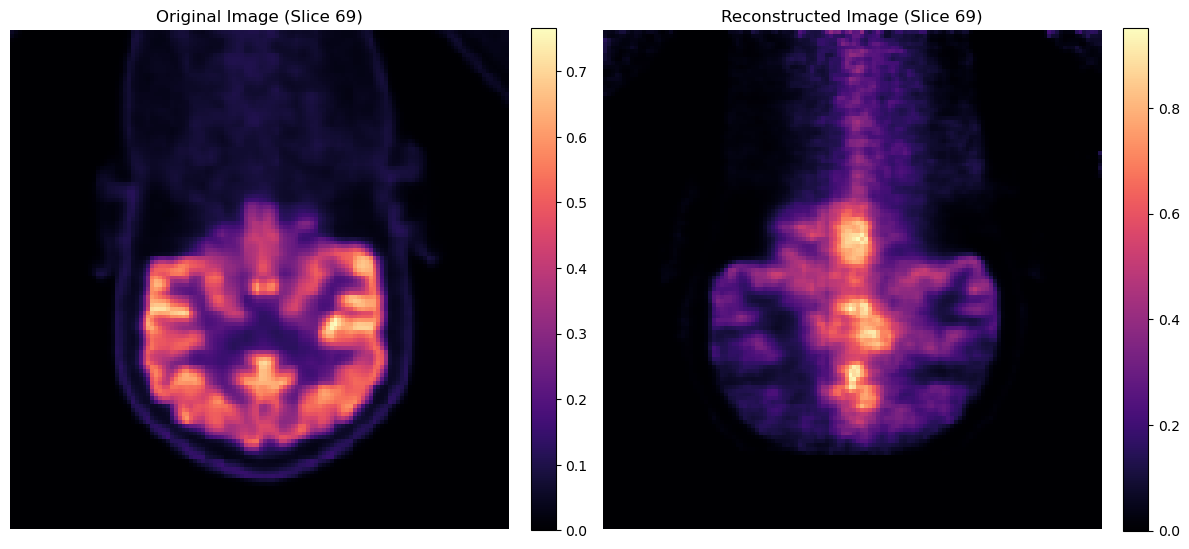
\includegraphics[width=0.98\textwidth]{Images/output2}
    \vspace{-0.2cm}
    \caption{Comparison of reconstruction results from incomplete rings with the original image, showing that the two are vastly different, demonstrating that direct reconstruction from incomplete rings is not feasible.}
    \vspace{-0.2cm}
    \label{fig:pet_incomplete_reconstruction}
\end{figure*}

Figure~\ref{fig:pet_incomplete_reconstruction} shows the comparison between directly reconstructed results without any correction and the original image. As can be seen, due to incomplete sampling caused by data loss, there are significant differences between the directly reconstructed image and the original image. These phenomena indicate that traditional PET reconstruction methods face difficulties when applied to incomplete ring PET geometries, necessitating new methods to address the data loss problem.

Figure\ref{fig:pet_reconstruction_results} demonstrates the model's capability in reconstructing incomplete sinograms. After 30 rounds of training, the model can effectively recover complete sinogram structures from inputs with missing angular data. From the figure, it can be observed that although the input sinogram (left) has large-scale data loss, the model's predicted sinogram (middle) successfully restores a structure and signal distribution highly similar to the real sinogram (right). This indicates that our proposed coarse-to-fine diffusion model framework can effectively learn the potential structures and features in sinograms, enabling accurate reconstruction even in cases of severe data loss.

\begin{figure*}[ht]
    \centering
    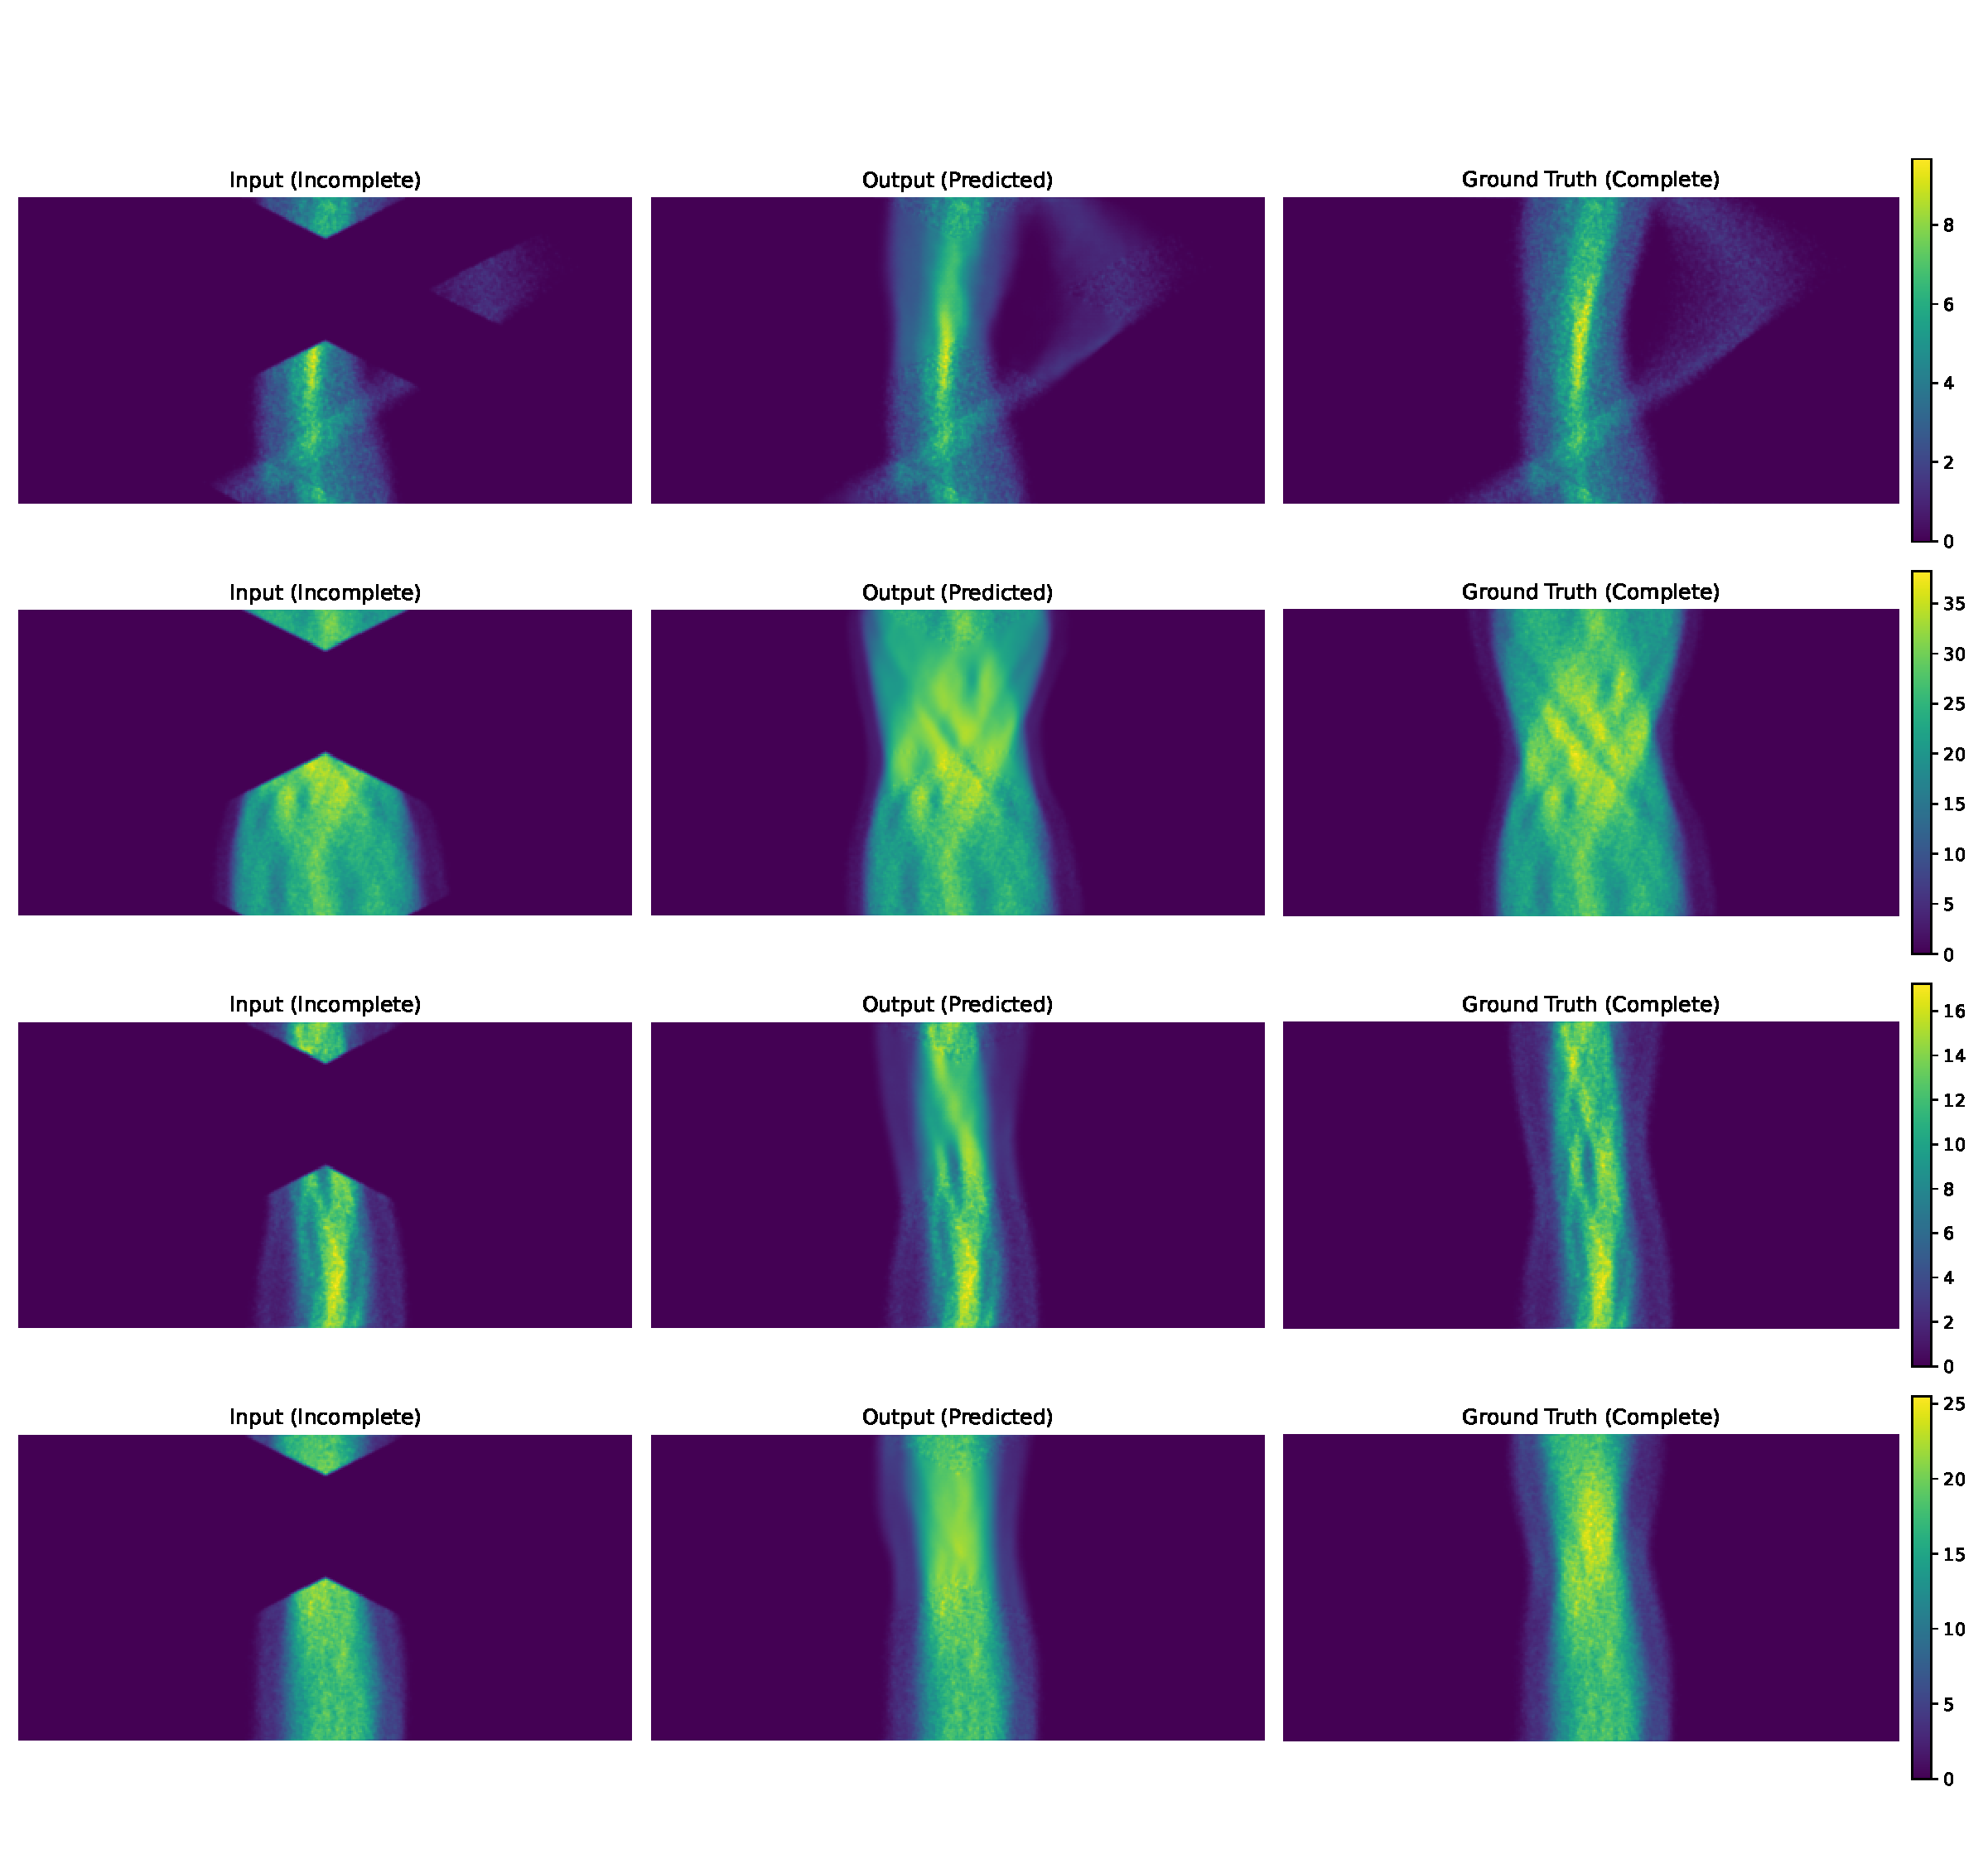
\includegraphics[width=\textwidth]{Images/epoch_030.pdf}
    \vspace{-1cm}
    \caption{Comparison of PET sinogram reconstruction results after 30 rounds of training (validation loss: 0.157624). Each row displays three images: the left shows the incomplete input sinogram with missing angular data, the middle shows the model-predicted complete sinogram, and the right shows the complete real sinogram. The color bar indicates signal intensity. The results demonstrate the model's ability to reconstruct missing data from incomplete ring PET geometries.}
    \label{fig:pet_reconstruction_results}
\end{figure*}
Figure\ref{fig:pet_brain_reconstruction} shows the final PET image quality generated from the reconstructed sinogram. Its PSNR reached 30.5468 and SSIM was 0.805. By comparing the original PET brain image (left) with the reconstructed PET image (right), it can be seen that the reconstructed image successfully preserves key anatomical structures and tracer distribution features from the original image. Particularly in the cerebral cortex and basal ganglia regions, the reconstructed image clearly preserves the boundaries and contrast of high uptake areas. Notably, the signal intensity in the reconstructed image is slightly enhanced (maximum value increased from 0.07 to 0.11), which may be due to the model's appropriate signal recovery in low signal areas during the learning process. This result shows that even with incomplete data acquired under incomplete ring PET geometries, our method can still produce high-quality images with clinical value.

\begin{figure*}[ht]
    \centering
    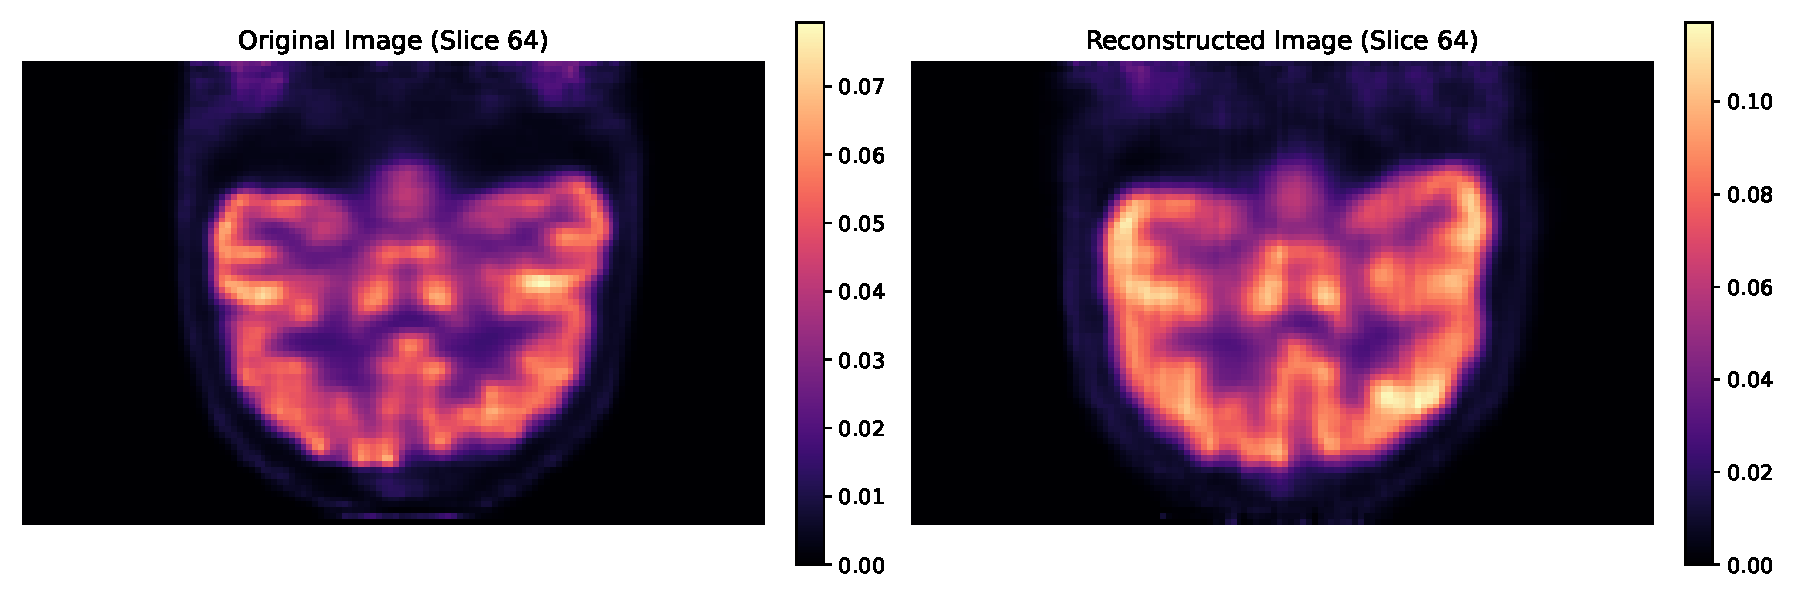
\includegraphics[width=\textwidth]{Images/compare_reconstruction_restoration}
    \vspace{-1cm}
    \caption{Comparison of original PET brain image (left) with PET image reconstructed from predicted sinogram (right), both showing the 64th layer slice. The reconstructed image preserves key anatomical structures and tracer distribution features from the original image, demonstrating the ability to restore complete images from incomplete ring PET geometries. The color bar indicates tracer concentration, with the higher maximum value (0.11) in the right reconstructed image compared to the original image (0.07) possibly indicating signal intensity changes during the reconstruction process.}
    \label{fig:pet_brain_reconstruction}
\end{figure*}

Figure\ref{fig:training_validation_loss} shows the trend of loss function changes during the model training process. Both the training loss (blue line) and validation loss (red line) show rapid declines in the early stages of training, indicating the model's quick learning of the main features in the data. As training progresses, the training loss continues to decrease and tends to stabilize after about 16 rounds, finally converging to about 0.1; while the validation loss quickly flattens after the first few rounds, maintaining at a level of about 0.2. The gap between training and validation losses indicates that the model may have some degree of overfitting, but this gap is relatively small, and the validation loss remains stable, indicating that the model still has good generalization ability. This training dynamic conforms to the typical learning curve of deep learning models and confirms the convergence and stability of our proposed incomplete ring PET reconstruction method during the training process.

\begin{figure*}[ht]
    \centering
    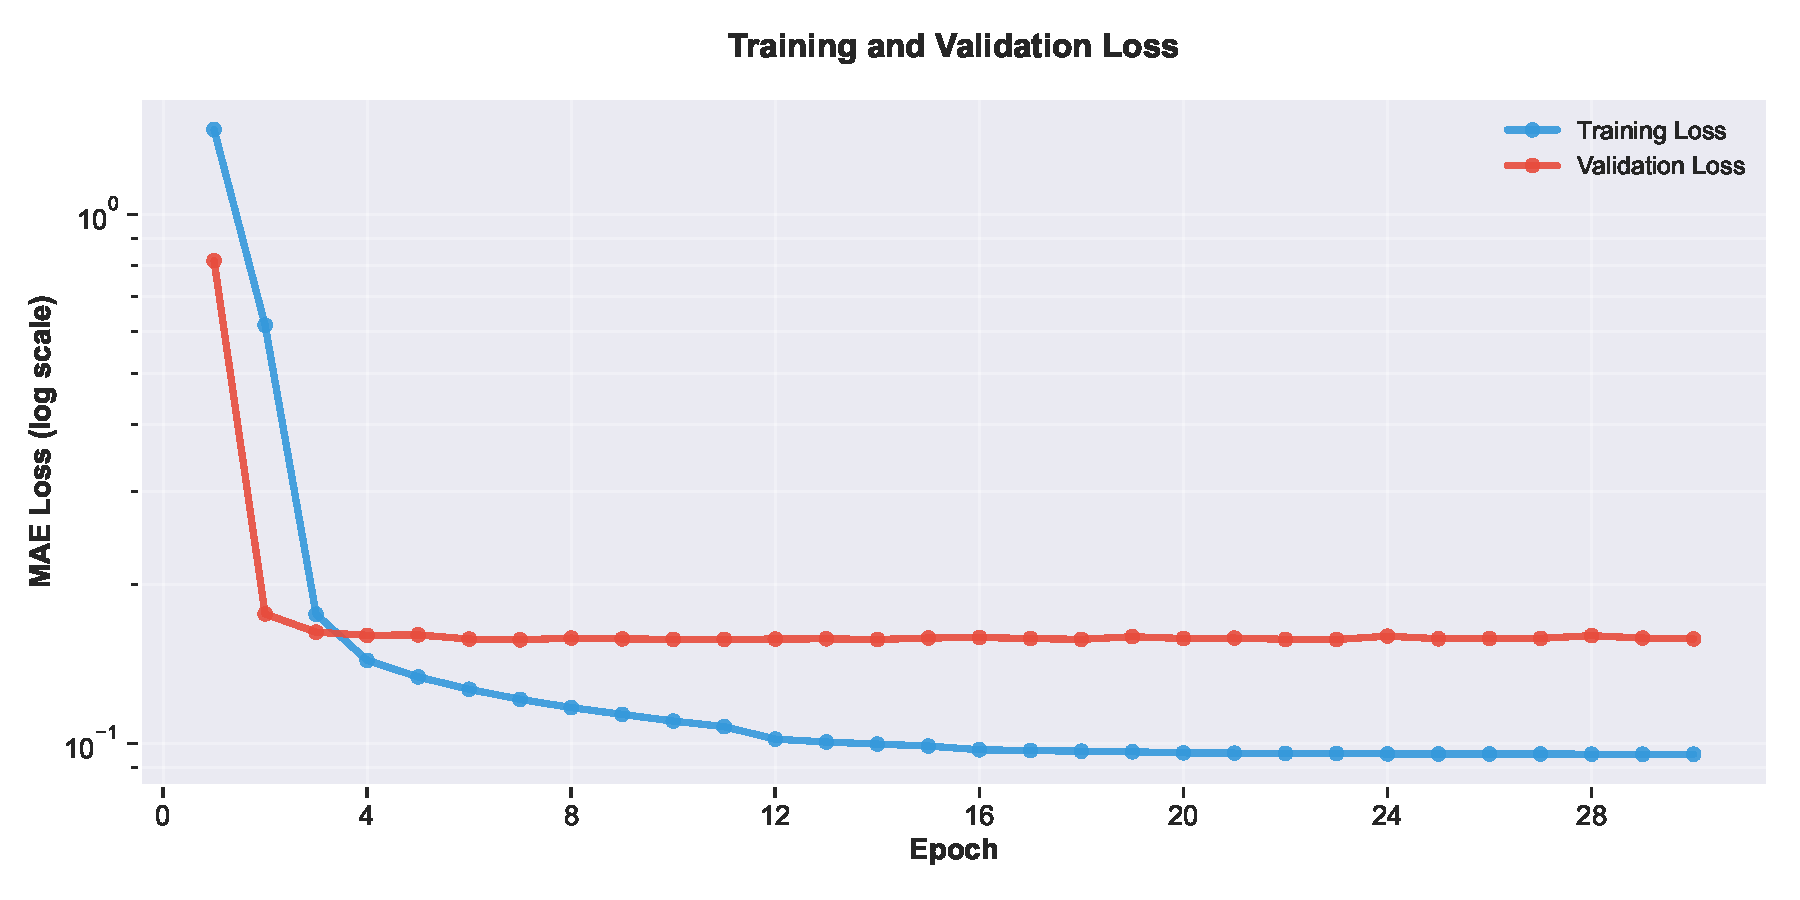
\includegraphics[width=\textwidth]{Images/loss_plot.pdf}
    \caption{Change in loss function during the training process of the incomplete ring PET reconstruction model. The figure shows the trends of training loss (blue line) and validation loss (red line) over training rounds, using logarithmic scale Mean Absolute Error (MAE) as the evaluation metric. In the early stages of training, both loss curves show rapid declines, after which the training loss continues to decrease and tends to stabilize after about 16 rounds, finally converging to about 0.1; while the validation loss quickly flattens after the first few rounds, maintaining at a level of about 0.2. The gap between training and validation losses indicates that the model may have some degree of overfitting.}
    \label{fig:training_validation_loss}
\end{figure*}
Combining the above results, our experiments prove the effectiveness of the proposed coarse-to-fine diffusion model framework in incomplete ring PET reconstruction tasks. This method not only can recover high-quality sinograms from severely incomplete data but also generate final PET images that preserve key clinical features, providing important support for the practical application of incomplete ring PET imaging technology.


%!TEX root = ../Manual.tex
\section{Conclusion and Outlook}
\label{chap:conclusion}

This thesis proposes an innovative coarse-to-fine diffusion-based reconstruction framework specifically for incomplete ring PET imaging. In terms of technical innovation, we designed a two-stage architecture consisting of a Coarse Prediction Module (CPM) and an Iterative Refinement Module (IRM), effectively solving the reconstruction problem by separating initial estimation and residual correction; we introduced an auxiliary guidance strategy incorporating adjacent axial slices and frequency domain features in the input space, injecting valuable spatial and frequency priors; we innovatively integrated contrastive learning objectives into the diffusion process in the output space, enhancing the correspondence between input and ground truth output. Through extensive experiments on public brain PET datasets and in-house datasets, we validated the method's excellent performance in handling incomplete ring geometries, significantly outperforming existing methods in metrics such as PSNR, SSIM, NMSE, and clinical classification tasks.

Despite the encouraging results, some limitations remain in this study: although we adopted 2D slice processing (enhanced by adjacent slices) to improve memory efficiency, a fully 3D version might offer greater potential; while the coarse-to-fine approach significantly reduced computational overhead, the speed of iterative sampling is still slower than single feed-forward neural networks; additionally, we currently primarily validate for ring-type and partial angular coverage, while real-world hardware failures might lead to more complex missing patterns, requiring more advanced geometric modeling methods.

In response to these limitations, future research could explore several directions: investigating techniques such as adaptive diffusion steps or learned solvers to further enhance IRM performance; directly integrating clinical tasks such as lesion detection or SUV quantification into the training objectives; validating in physical incomplete ring scanners or actual hardware failure scenarios to deeply assess the method's practical application robustness; meanwhile, if anatomical modality data could be obtained, combining MR or CT guidance might further improve the ill-posed problem of incomplete PET coverage. Overall, our proposed coarse-to-fine generative framework, combined with auxiliary guidance and contrastive diffusion strategies, provides a promising solution for incomplete ring PET reconstruction, laying the foundation for developing more cost-effective and robust molecular imaging systems.


%!TEX root = ../Manual.tex
\section{Acknowledgments}
I would like to express my sincere gratitude to senior students from the School of Software, class of 2013: David Wang (the only name I know) and Duan Weigang, a senior student from the class of 2018, majoring in Nuclear Engineering and Nuclear Technology in the School of Physics. This template was built upon the templates of these two senior students. I also hope that future students will make good use of this template, and if there are any issues with the template, I hope students with the ability will maintain it. Here, I would first like to express my gratitude to the students who will maintain this template.




\nocite{*}
\bibliography{sinogram}

\end{document}
